%% file: VaBlaetter.tex
%% author: Martin Koelbl
%% date: 1.08.2015
%% purpose: Va-Blaetter Herbst 2015 Hauptdatei

%% Flag, das anzeigt, ob vorlaeufige oder final-Version erstellt wird:
\newif\ifDraft\Draftfalse

%% Flag das anzeigt ob eine Kurzversion erstellt wird:
%% Kurzversion derzeit noch kaum implementiert.
\newif\ifKurzversion\Kurzversionfalse
%\Kurzversiontrue
%% Flag das anzeigt ob Links erstellt werden:
%% Vorsicht: Wenn \Linksfalse eingestellt wird, dann die Datei fktana.ind loeschen und neu erstellen (mit makeindex), sonst beisst sich LaTeX die Zaehne aus.
\newif\ifLinks\Linkstrue
%\Linksfalse


%% Umgebungs-Einstellungen laden, falls vorhanden:
\InputIfFileExists{env_settings.tex}{}{}

%% Dokument-Beschreibung:
%% file: header.tex
%% author: Patrick Leyendecker
%% date: 23.08.2012
%% purpose: Va-Blätter Header nach Vorlage des Skriptenprojekts

\ifDraft
  \global\def\Draftoption{,draft}
\else
  \global\def\Draftoption{}
\fi
%\documentclass[a4paper,12pt,ngerman\Draftoption,twoside]{scrartcl}%,\driver
\documentclass[a4paper,12pt,ngerman,twoside]{scrartcl}

\usepackage[utf8]{inputenc}
%\usepackage[OT2, T1]{fontenc}
\usepackage[ngerman]{babel}

\usepackage{fancyhdr}
\usepackage{amsmath}
\usepackage{xcolor}
\usepackage{graphicx}
\usepackage{paracol}

\usepackage[inner=22mm, outer=26mm, bottom=0mm, top=0mm,footskip=40mm]{geometry}  
\usepackage{textcomp}

 % Seiten-Layout
\usepackage{verbatim}
\usepackage{array}
\usepackage{multicol}
\usepackage{multirow}
\usepackage{eurosym}
\usepackage{blindtext}
\usepackage{lipsum}
\usepackage{soul}
%\usepackage{ulem}
\usepackage{wrapfig}
\usepackage[absolute]{textpos} 
\usepackage{subfigure}
\usepackage{caption}
%\usepackage{subcaption}
\usepackage{dblfloatfix}

%\usepackage{cyrillic}
\usepackage{graphicx}
\newcommand{\heart}{\ensuremath\heartsuit}

\geometry{vmargin={3cm,4cm}}


\makeatother
%% subsubsections nicht mehr nummerieren:
\setcounter{secnumdepth}{1}
%% subsubsections nicht ins Inhaltsverzeichnis:
\setcounter{tocdepth}{1}

\setlength{\parindent}{0pt}

%% Nummerierung von Abbildungen und Tabellen:
\numberwithin{figure}{section}
\numberwithin{table}{section}

\addtokomafont{caption}{\itshape}
\renewcommand*{\figureformat}{}
\renewcommand*{\captionformat}{}

\setlength{\headheight}{26pt}

\setlength{\columnsep}{30pt}

\setlength{\parskip}{6pt}

% Disable single lines at the start of a paragraph (Schusterjungen)
\clubpenalty = 10
%
% Disable single lines at the end of a paragraph (Hurenkinder)
\widowpenalty = 10000
\displaywidowpenalty = 10




\pagestyle{fancy}
% \fancyfoot{}
\fancyhead{}
\fancyhead[EL,OR]{ \footnotesize Seite \thepage \\ Die Vandalenblätter}
\fancyhead[ER,OL]{\footnotesize 130/2025 } %\\ (Nummer 32 -- Herbst
% 2014)}
\fancyhead[EC,OC]{ \large \textsc{\leftmark } \vspace{0pt}}

\renewcommand{\thesection}{}
\renewcommand{\theparagraph}{}
\renewcommand{\thesubsubsection}{}
\renewcommand{\sectionmark}[1]{\markboth{#1}{}}

\makeatletter
\newenvironment{tablehere}
  {\def\@captype{table}}
  {}

\newenvironment{figurehere}
  {\def\@captype{figure}}
  {}
\makeatother


%% Makros und Umgebungen:
%%% file: makros.tex
%% author: Thomas Satzger
%% date: 08.03.2007
%% purpose: Diplomarbeit, LaTeX-Definitionen


%% Theorem-Umgebungen:

%% Nummerierung nach sections, alle Theoreme mit dem gleichen Zaehler:
\theorembodyfont{\rmfamily}
\theoremstyle{break}% neue Zeile nach Theoremueberschrift
\newtheorem{defi}{Definition}[section]
\newtheorem{lemma}[defi]{Lemma}
\newtheorem{satz}[defi]{Satz}
\newtheorem{kor}[defi]{Korollar}
\newtheorem{bem}[defi]{Bemerkung}
\newtheorem{bemerkung}[defi]{Bemerkung}
\newtheorem{bemerkungen}[defi]{Bemerkungen}
\newtheorem{beispiel}[defi]{Beispiel}
\newtheorem{beispiele}[defi]{Beispiele}
\newtheorem{nothing}[defi]{\hspace{-1ex}}% Umgebung ohne Ueberschrift
%% TODO: nothing schaut furchtbar aus.


%% Umgebungen ohne Nummer:
% \input thbnone.sty
% \theoremstyle{bnone}% wie break, nur ohne Nummer
%\newtheorem{defi*}{Definition ohne Nummer}[section]
\newtheorem{beispiel*}{Beispiel}[section]
\newtheorem{beispiele*}{Beispiele}[section]
\newtheorem{bem*}[beispiel*]{Bemerkung}
\newtheorem{bemerkung*}[beispiel*]{Bemerkung}
\newtheorem{bemerkungen*}[beispiel*]{Bemerkungen}
\newtheorem{folgerung}[beispiel*]{Folgerung}
\newtheorem{folgerungen}[beispiel*]{Folgerungen}
%% Beweis:
%% qed-Kaestchen wird automatisch gesetzt, ausser es wurde schon 
%% von Hand (per \qed) gesetzt.
%% Ist eine Liste am Ende vom Beweis (d.h. itemize/enumerate/description),
%% dann muss \qed nach dem letzten Text (von Hand) eingefuegt werden.
\newtheorem{beweis}[beispiel*]{Beweis}
\let\tmpendbeweis=\endbeweis
\def\endbeweis{\smartqed\tmpendbeweis}


%% QED-Kasterl. Am sinnvollsten am Ende eine Absatzes
%% Klappt im Mathemodus nicht so toll.
\newif\ifQed\Qedfalse % speichern, ob manuell qed gesagt wurde 
%% (damit bei \end{beweis} nicht noch ein qed dazu kommt)
\newcommand{\qed}{\nolinebreak[4]\hfill\rule{1.2ex}{1.2ex}\global\Qedtrue}% 
%% qed, dass nur bei \Qedfalse gesetzt wird (fuer Beweisumgebung):
\newcommand{\smartqed}{\ifQed\relax\else\qed\fi\global\Qedfalse}


%% Keine Beweise, Beispiele in der Kurzversion:
%% TODO: Hier kann man noch optimieren (Beispiele rauslassen geht noch nicht).
\ifKurzversion
  \let\beweis=\comment
  \let\endbeweis=\endcomment
\fi


%% enumerate- und itemize-Umgebungen anpassen:
\partopsep=-\parskip% wirkt bei Absaetzen vor enumerate
\let\tmpenumerate\enumerate
\def\enumerate{\par%\vspace{-\topsep}
\vspace{-\parskip}%
\vspace{-\partopsep}%
\tmpenumerate\partopsep=0mm\itemsep=0mm\parsep=0mm}

%% Zwei neue Umgebungen f�r Listen: lista mit Buchstabenz�hlung, und listi mit r�mischen Zahlen
%% muss noch entwickelt werden
\newcommand{\listea}{\begin{enumerate}[\medspace (a)]}
\newcommand{\listeaend}{\end{enumerate}}
\newcommand{\listei}{\begin{enumerate}[\medspace $(i)$]}
\newcommand{\listeiend}{\end{enumerate}}
\newcommand{\liste}{\begin{enumerate}[\medspace 1.]}
\newcommand{\listeend}{\end{enumerate}}

\newcommand{\nobr}{\nolinebreak}

\newcommand{\vo}{ v\//\/o }


%Operatoren
%\DeclareMathOperator{\rang}{rang}
%\DeclareMathOperator{\sgn}{sgn}

% \vecn - Allgemeiner 1xn-Spaltenvektor mit Klammern ausnrum
% F�r Zeilenvektoren nimmt man besser \mat (siehe unten)
% Beispiel: \vecn{a \\ b \\ c}
%\newcommand{\vecn}[1]
%{\left(\begin{array}{c} #1 \end{array}\right)}

% \closure{TEXT} macht einen �berstrich �ber den TEXT,
% Denke an den Abschluss von Mengen
\newcommand{\closure}[1]
{\overline{#1}}

% \mat{SPALTEN}{INHALT} - Matrizen (mit normalen  ( ) )
% Beispiel: \mat{cc}{a & b \\ c & d}
\newcommand{\mat}[2]
{\left(\begin{array}{#1} #2 \end{array}\right)}

% \detmat{SPALTEN}{INHALT} - Determinanten-Matrizen ( | | statt ( ) )
% Syntax wie bei \mat
%\newcommand{\detmat}[2] % det ist leider vergeben
%{\left|\begin{array}{#1} #2 \end{array}\right|}

% \gmat{SPALTEN}{INHALT} - Matrizen mit geschweiften Klammern ( { } statt ( ) )
% Syntax wie bei \mat
\newcommand{\gmat}[2] % det ist leider vergeben
{\left\{\begin{array}{#1} #2 \end{array}\right\}}


%% Skalarprodukt:
%% Das Argument steht zwischen den Klammern.
\def\skalar#1{\ensuremath{\left\langle #1\right\rangle}}

%% Absolutbetrag (einfache senkrechte Striche, 
%% Groesse automatisch angepasst):
%% TODO: In chapter2.tex ab section 5 einfuegen.
\newcommand{\abs}[1]{\ensuremath{\left|#1\right|}}

%% Norm (doppelte senkrechte Striche, Groesse automatisch angepasst):
\def\norm#1{\ensuremath{\left\|#1\right\|}}

%% Erzeugendensystem einfach und doppelt
\def\erz#1{\ensuremath{\left\langle #1\right\rangle}}
\def\erzerz#1{\ensuremath{\left\langle\left\langle #1\right\rangle\right\rangle}}

%% Stacked Equal: = mit einem mathrm-Text dr�ber
\newcommand{\smequals}[1]
{\stackrel{\mbox{\tiny #1}}{=}}

\newcommand{\smany}[2]
{\stackrel{\mbox{\tiny #1}}{#2}}


% Personen-Namen werden in guten B�cher in Kapit�lchen geschrieben
\newcommand{\name}[1]{\textsc{#1}}


%% Mathe-Pfeile:
% Langer �quivalenzpfeil mit Abst�nden:
\def\aequiv{\ensuremath{\ \Longleftrightarrow\ }\xspace}
% Langer Implikationspfeil mit Abst�nden:
\def\impl{\ensuremath{\ \Longrightarrow\ }\xspace}
% Definitions�quivalenzpfeil mit Abst�nden:
\def\define{\ensuremath{\ :\Longleftrightarrow\ }\xspace}
% Beweis, Hin-Richtung und R�ck-Richtung:
% Verwendung: 
%\begin{description}\item[\hin]...\item[\rueck]...\end{description}
\def\hin{\glqq$\Longrightarrow$\grqq{}}
\def\rueck{\glqq$\Longleftarrow$\grqq{}}
% Geschweifte Klammer mit Kommentar unter Formeln:
% Zuerst den tiefgestellten Text, dann den normalen.
\def\underbraced#1#2{\ensuremath{\underset{\rule{0mm}{1.5ex}\makebox[0mm]{$\scriptstyle #1$}}{\underbrace{#2}}}}
% Transponiert:
%\def\trans{^{\mathsf T}}
\def\trans{^{\mathrm T}}

% Orthogonal
\def\ortho{^{\bot}}


%% TODO-Makro:
\def\todo#1{\ifDraft\par{\bfseries TODO: #1}\par\fi}
%% Marke zum Bild einfuegen, Argument ist z.B. Bildbeschreibung (caption):
\def\bild#1{\todo{Bild: #1}}


%% Makros spezifisch fuer Funktionalanalysis:
% Topologie (Schreibschrift-T):
\def\topo{\ensuremath{\mathcal T}}
% Bidual: Setzt zwei hochgestellte Sterne.
\def\bidual{\ensuremath{^{\ast\ast}}}

% URL einf�gen
\DeclareRobustCommand{\urlformat}[1]{\url{#1}} 

%% Bilder einfuegen:
%% Syntax:
%%   \abbildung{dateiname}[graphicx-optionen]{Beschriftung}[label]
%% Argumente: Dateiname (ohne Pfad und Endung), 
%% Optionen fuer includegraphics (optional), 
%% caption, Label (optional).
%% Beispiele:
%% \abbildung{hausdorff}{Zur Hausdorff-Eigenschaft}
%% \abbildung{hausdorff}{Zur Hausdorff-Eigenschaft}[fig:hausdorff]
%% \abbildung{hausdorff}[height=5cm,width=\textwidth,keepaspectratio=]{Zur Hausdorff-Eigenschaft}
\def\bilderpfad{./bilder/}
%\ifthenelse{\equal{\driver}{pdftex}}%
%  {\global\def\bildendung{.pdf}}%
%  {\global\def\bildendung{.ps}}% 
\makeatletter
\def\abbildung#1{\@ifnextchar[{\@bbildung{#1}}{\@bbildung{#1}[scale=1]}}
\def\@bbildung#1[#2]#3{%
  \@ifnextchar[{\@bbild@ngl{#1}[#2]{#3}}{\@bbild@ng{#1}[#2]{#3}}}
\def\@bbild@ng#1[#2]#3{%
  \begin{figure}[htb]
    \begin{center}
      \includegraphics[#2]{\bilderpfad#1}%\bildendung
      \caption{#3}
    \end{center}
  \end{figure}}
\def\@bbild@ngl#1[#2]#3[#4]{%
  \begin{figure}[htb]
    \begin{center}
      \includegraphics[#2]{\bilderpfad#1}%\bildendung
      \caption{#3}
      \label{#4}
    \end{center}
  \end{figure}}
\makeatother




\def\Input{\item[\textbf{Input: }]}
\def\Output{\item[\textbf{Output: }]}
\def\comment{\%}
\def\Given{\item[\textbf{Gegeben: }]}
\def\False{\ensuremath{\text{\bfseries False}}}
\def\True{\ensuremath{\text{\bfseries True}}}
\def\return{\ensuremath{\text{\bfseries Return}}}

\def\var#1{\ensuremath{\textit{#1}}}
%\renewcommand\algorithmiccomment[1]{ \{#1\}}%


\renewcommand\appendix{\par
\setcounter{section}{0}%
\setcounter{subsection}{0}%
\setcounter{figure}{0}
\renewcommand\thesection{\Alph{section}} %
\renewcommand\thefigure{\Alph{section}.\ arabic{figure}}} 



%% Zwei neue Umgebungen für Listen: lista mit Buchstabenzählung, und listi mit römischen Zahlen
%% muss noch entwickelt werden
% \newcommand{\listea}{\begin{enumerate}[\medspace (a)]}
% \newcommand{\listeaend}{\end{enumerate}}
% \newcommand{\listei}{\begin{enumerate}[\medspace $(i)$]}
% \newcommand{\listeiend}{\end{enumerate}}
% \newcommand{\liste}{\begin{enumerate}[\mAnonymer Barbetriebedspace 1.]}
% \newcommand{\listeend}{\end{enumerate}}

\newcommand{\nobr}{\nolinebreak}
\newcommand{\vo}{v\//\/o }
%\newcommand{\tocline}[1]{\addtocontents{toc}{\contentsline {section}{\numberline{}{\hspace{-0.5cm}{\large {#1}}}}}}
\newcommand{\tocline}[1]{\addtocontents{toc}{section}{\numberline{}\hspace{-0.5cm}{\large {#1}}}}
% select ONE of the two following lines to switch between color and bw pictures
\newcommand{\Bilder}{Bilder}
%\newcommand{\Bilder}{Bilder/farbig}

\newcolumntype{P}[1]{>{\centering\arraybackslash}p{#1}}


%\makeindex
\pagenumbering{arabic}


\begin{document}

%% Titelseite:

\begin{titlepage}

%\Huge Dummy für Titelseite

\begin{textblock}{3}(0,0) 
     \includegraphics[width=1.\paperwidth]{Titelseite/130Titlepage}
\end{textblock} 

\end{titlepage}

\leavevmode\newpage


%% Disclaimer:
%\input disclaimer.tex

\clearpage


%% Inhaltsverzeichnis:
%\linespread{1}

% Zeilenabstand im Inhaltsverzeichnis:
\addtocontents{toc}{\protect\linespread{+0.2}\protect\selectfont}

\tableofcontents
\enlargethispage{1cm}

\clearpage


%%%%%%%%%%%%%%%%%%%%%%%%%%%%%%%%%%%%%%%%%%%%%%%%%
%% Teil WS1819

%\section*{Wintersemester 2024/2025}
\sectionmark{Impressum}

\enlargethispage{1cm}

%\vspace*{5mm}
\begin{figurehere}
 \begin{center}
   %\includegraphics[width=0.8\hsize]{Bilder/chargen/chargen3.JPG}
   \includegraphics[width=0.8\hsize]{Bilder/chargen/chargen3.jpg}
   
   \caption{Das Chargenkabinett des WS 24/25}
 \end{center}
\end{figurehere}

%\vspace*{.5cm}

%\textbf{Chargenkabinett des WS 2024/2025} \vspace*{1cm} \\
\vbox{
	\begin{tabular}[h]{*5{c}}
		Scriptor & Fuxmajor & Senior & Consenior & Kassier\\
		\textbf{Benedikt Kirchhof} & \textbf{Magnus Weig} & \textbf{Raphael Frank} & \textbf{Elia Strasser} & \textbf{Felix Hantke} \\
		\textit{stud. paed.} & \textit{stud. el.} & \textit{stud. inf.} & \textit{stud. rer. oec.} & \textit{stud.paed.}\\
	\end{tabular}
}

\vspace{2mm}
%\subsection*{Semestermotto des WS 2024/2025}
\begin{LARGE}
	\begin{center}
		\glqq Wer nichts weiß, muss alles glauben\grqq
	\end{center}
%	\hspace*{2cm}\glqq Tradition soll ein Sprungbrett sein,\\
%    \hspace*{7cm} aber kein Ruhekissen.\grqq
\end{LARGE}

\vspace*{-3mm}
- \textit{Marie von Ebner-Eschenbach}

\vspace*{7mm}
\begin{minipage}[h!]{160mm}
	\small{
		\textbf{Impressum}
		
		Vandalenblätter 130/2025, Ausgabe WS 2024/25
		
		Mitteilungsblatt der K.D.St.V. Vandalia Prag zu München im CV
		
		Namentlich gekennzeichnete Beiträge stellen keine redaktionelle Meinungsäußerung dar. Die Redaktion behält sich vor, Änderungen vorzunehmen, die den Sinn des Textes wahren.
		\\
		\newline
		\vspace{6pt}
		\noindent\begin{tabular}{ll}
			Titelbild: & Philipp Keyzman\\
			Lizenz: & Creative Commons 2.0 \\
			Satz \& Layout: & Philipp Keyzman, Alessandro Samuelli und Leonard Rothe mittels
			\LaTeX
			\\
			Bildmaterial: & Elias Haindl\\
			Druck: & https://www.wir-machen-druck.de\\
			Auflage: & 500 Stück\\
			Redaktionsanschrift: & Vandalenblätter-Redaktion \\	
			& c/o K.D.St.V. Vandalia\\
			& Friedrichstraße 34, 80801 München\\
			& vablaetter@vandalia.de
		\end{tabular}
	}
	
\end{minipage}
\clearpage

\clearpage


%%%%%%%%%%%%%%%%%%%%%%%%%%%%%%%%%%%%%%%%%
%% Vorworte

\section{Vorwort des Philisterseniors}
\sectionmark{Vorwort des Philisterseniors}

%\begin{figurehere}
%	\begin{center}
%		\includegraphics[width=\linewidth]{Bilder/andechs2.jpg}
%%		\caption{xxx} 
%	\end{center}
%\end{figurehere}

\begin{multicols}{2}

Die Jahreshauptversammlung des CV fand in diesem Jahr in Berlin statt. Sie war geprägt durch eine Diskussion über unser Prinzip religio. Der ein oder andere hat davon vielleicht in der ACADEMIA etwas gelesen. Die Diskussionen waren auch in den vorausgegangenen Regionaltagungen zum Teil sehr hitzig. Ohne die Details hier auszubreiten, möchte ich aber einen kurzen Blick darauf werfen. Die Tatsache, dass ein Vorort seine Amtszeit dadurch prägen will, etwas zu verändern und dann nicht bis zur CV damit wartet, sondern bereits zu Beginn seiner Amtszeit einen Diskurs startet, halte ich für richtig. Jedes Chargenkabinett - sei es im Vorort oder auch in der Verbindung - hat eine zeitlich begrenzte Amtszeit. Veränderungsprozesse am Ende der Amtszeit zu starten, sind zumeist sinnlos. Aus dieser Sicht betrachtet, war das Vorgehen des Vororts Berlin sehr gut geplant und kann und sollte ein Vorbild für zukünftige Chargenkabinette sein.
Über den Inhalt wird und wurde trefflich diskutiert und gestritten. Aus meiner Sicht gibt es hier durchaus gute Impulse. Über andere Thesen darf und muss man auch geteilter Meinung sein. Wichtig scheint mir aber, dass wir Themen und auch unsere Prinzipien diskutieren. Ohne Diskussion über unsere Prinzipien und wie wir sie auch in Zukunft leben, stellt sich jedem von uns über kurz oder lang die Frage nach der Bedeutsamkeit unseres Verbandes.
Gute Diskussionen über strittige Themen können verbinden, das Profil stärken und sollten uns als akademischen und katholischen Verband ausmachen. Als wichtige und beruhigende Botschaft aus diesen Diskussionen ist mir unser einigendes Motto immer wieder lebendig vor Augen geführt worden: \glqq In necessariis unitas, in dubiis libertas, in omnibus caritas\grqq!
Der zentrale Punkt ist mir aber, dass hinter diesen Diskussionen spürbar ist, dass es Cartellbrüder gibt, denen unser Verband und unsere Verbindungen wichtig sind. Heute ist das für mich ein stärkender Impuls entgegen der weitverbreiteten Egozentrik und Selbstoptimierung in unserer Gesellschaft.
Ich würde mich freuen, wenn wir auch im Jahr unseres 120. Gründungs- und Stiftungsfests aktiv über die Weiterentwicklung unserer Vandalia sprechen und diskutieren. Was bedeuten unsere Prinzipien für uns auch im 21. Jahrhundert! Diese Auseinandersetzung in bundesbrüderlicher Freundschaft ist für ein “vivat, crescat, floreat at multos annos Vandalia” unbedingt notwendig! 

\end{multicols}
\begin{flushright}
		\hfill\emph{Dr. Michael Spickenreuther Va!}
	\end{flushright}
\newpage

\section{Vorwort des Seniors aus dem WS 2023/24}
\sectionmark{Vorwort des Seniors}

Liebe Freunde der Vandalia,\\
Liebe Bundesbrüder,
\begin{multicols}{2}

Es ist mir eine Freude, Dir die neuste Ausgabe der Vandalenblätter vorstellen zu dürfen. Dank gilt dabei vor allem den Redakteuren dieser Ausgabe, den Bundesbrüdern Philipp Keyzman und Benedikt Kirchhof, welche diese Ausgabe zusammengestellt haben und gegen viele Widrigkeiten die Prozesse, die hierfür notwendig sind, wiederbelebt oder gar neu erfunden haben. So hoffe ich, dass die Artikel Dir einen guten Einblick in das vergangene Wintersemester geben können und auch bei den Bundesbrüdern, welche daran aktiv teilgenommen haben, so manche schöne Erinnerung wieder hervorruft. An dieser Stelle möchte ich - auch stellvertretend für die Redaktur - Dich nochmal herzlich dazu einladen, gerne auch Deine eigenen Beiträge einzusenden. Ob Du aus Deiner akademischen Arbeit, Deinem Alltag, einer spannenden Reise berichten oder einfach einen Kommentar zum aktuellen Geschehen in der Verbindung und Welt verfassen möchtest: Gerne nehmen wir diese Artikel oder auch photographischen Interpretationen in die Blätter auf und fördern so den Austausch zwischen den Bundesbrüdern. Hierfür sind die Redakteure in Zukunft unter \textbf{vablaetter@vandalia.de} erreichbar, sodass die Artikel auch eine Amtsübergabe überdauern werden.

Zuletzt möchte ich Dir noch kurz die Chargen des vergangenen Wintersemesters 2023/24 vorstellen und anschließend einen kurzen Überblick über dieses geben. Als Kassier und Schriftführer konnten die Bundesbrüder Daniel Rampf und Raphael Frank erste Erfahrungen in der Chargenarbeit gewinnen. Sie wurden zusammen mit ihrem Leibbruder Elia Strasser auf dem Gründungsfestkommer geburscht. Die gesammelte Erfahrung prädestiniert sie dafür, in Zukunft auch höhere Verantwortung für unsere liebe Vandalia zu übernehmen. Als Fuxmajor kümmerte sich Bundesbruder Fabian Heinrich in seiner vierten Charge um die Keilarbeit sowie die Erziehung des Fuxenstalls. Der Hohe Consenior, Bundesbruder Derek Dominguez, kam im WS 2022/23 als ZM zu unserer Vandalia. Zuvor besuchte er in Hamburg das Studienkolleg und wurde im WS 2021/22 bei e.V. K.D.St.V. Wiking Hamburg rezipiert. Er bereicherte das Semester und insbesondere die Begrüßungsabende durch Gerichte aus seiner ecuadorianischen Heimat. Als Senior durfte ich, Konrad Schönleber, wie bereits im Sommersemester unserer lieben Vandalia vorstehen.
\\
Das Semester stand unter dem Wahlspruch \textit{"Wo sich Männr finden, die für Ehr und Recht, mutig sich verbinden, weilt ein frei Geschlecht"}. Dieses Zitat aus dem Gedicht "Freiheit, die ich meine" von dem Dichter Max von Schenkendorf wurde etwa in einigen Kneipreden erörtert. Neben diesen obligatorischen Kneipen fand im Semester auch eine Rezeptionskneipe statt. Es wurden auf jenen Veranstaltungen sieben Füxe rezipiert, von welchen uns leider im Laufe des Semesters zwei verlassen mussten, sodass sich der Fuxenstall mit nun fünf Füxen doch adäquat gefüllt zeigt. Höhepunkt des Semesters war das vom 24. bis 26. November stattfindende 119. Gründungsfest. Dieses war herausragend besucht und wir hatten die Ehre, den 1. Vizepräsidenten aD des Bayrischen Landtags, Karl Freller hierzu als Festredner begrüßen zu dürfen. Das Grundprinzip der religio war unter anderem durch Besuche der Roratemessen oder auch dem Pater-Rupert-Mayer-Gedächtnisgottesdienst vertreten. Auch die scientia kam mit verschiedenen Vorträgen und Museumsbesuchen nicht zu kurz. Neben der Feuerzangenbowle fand auch eine familiäre Adventsfeier als eine winterliches Äquivalent des Maifests statt. Hierzu wurde zwar eine größere Menge an Gebäck gebacken, allerdings konnte sie wegen Krankheit vieler Bundesbrüder nur in recht kleinem Kreise stattfinden. Man könnte sie vermutlich in den kommenden Jahren mit wenig Aufwand zu einer größeren Veranstaltung ausbauen, wenn man dies den Bundesbrüdern besser kommunizieren würde. Anfang November gab es zudem schon ein frühes, kleines Feierwochenende: Bei einem zweitägigen Tanzkurs wurden die Kenntnisse der Bundesbrüder für die kommende Ballsaison aufgefrischt. Zudem durften wir uns an diesem Samstag den den Genuss einer Martinsgans kommen. Hierfür gilt mein Herzlicher Dank an Fbr. Rampf e.V. K.St.V. Rechberg sowie an seine Frau für die sehr lehrreiche Durchführung des Tanzkurses und an unsere Bundesbrüder AH Michael Oppitz sowie AH Richard Gurtner, welche das Martinsgansessen organisiert und mit bester Kochkunst vorbereitet haben.
Doch zu den einzelnen Veranstaltungen kannst Du in den folgenden Artikeln detailliertere und hoffentlich weniger langweilige Worte finden. So bleibt mir nur, meinen Dank an alle Bundesbrüder und insbesondere an die Philisterchargen für die Unterstützung vor und während des Semesters auszusprechen. Ich bin höchst erfreut, dass ich unserer Vandalia zwei Semester vorstehen durfte und hier in der schönsten Stadt am Isarstrande eine zweite Heimat in unserer Verbindung gewinnen konnte.  

Auf dass diese Freude noch vielen weiteren Bundesbrüdern zuteil werden wird:

Vivat, crescat, floreat Vandalia ad multos annos!
	%
	\begin{flushright}
		\hfill\emph{Konrad Schönleber RBo! Va!}
	\end{flushright}
	%
\end{multicols}


\clearpage

\newpage
\section{Kneipreden des WS 2023/24}
\sectionmark{Kneipreden des Wintersemesters 2023/24}

%\begin{figurehere}
%	\begin{center}
%		\includegraphics[width=\linewidth]{Bilder/andechs2.jpg}
%%		\caption{xxx} 
%	\end{center}
%\end{figurehere}

Liebe Bundesbrüder,

folgend habe ich Euch die Kneipreden aus dem vergangenen Semester zusammengeschrieben. Dies könnte insbesondere für die Bundesbrüder welche es leider nicht zu den Kneipen und dem Kommers geschafft haben, aber auch für diejenigen welche sie nochmal in Ruhe lesen möchten, interessant sein. Natürlich entsprechen die hier abgedruckten Reden nicht genau den auf der Kneipe Vorgetragenen. So habe zumindest ich einerseits bei diesen immer wieder mal auch spontane kleine Gedanken eingefügt. Und andererseits bin ich vor der Veröffentlichung hier nochmal über alle Texte drübergegangen, habe Rechtschreibung und Grammatik möglichst weit korrigiert und überschüssigen, langweiligen Ballast entfernt sowie Gedanken eindeutiger formuliert. Denn Intentionen und Aussagen, die man in einer Rede durch Gestik und Mimik unterstreichen kann, sind im Schrifttext schwerer zu fassen. So wünsche ich Euch viel Spaß beim Lesen und hoffe, dass die Texte Eure Gedanken anregen.
\\

\begin{multicols}{2}
\textbf{Rede des Seniors auf der Semesterantrittskneipe des Wintersemesters 2023/24:}

Werte Kneipcorona,
\\
im Jahre 1812 zogen gut eine halbe Millionen Mann über die Memel und bis in das zerstörte Moskau, bevor die Grande Armee Napoleons den russischen Weiten und Winter erlag und damit das Ende dessen Herrschaft über weite Teile der deutschen Lande bedeutete.
Vor ziemlich genau 210 Jahren, vom 16. bis 19. Oktober, besiegten die Alliierten in der Völkerschlacht von Leipzig die bis dahin unbesiegte französische Armee.
In Deutschland herrschte eine hoffnungsvolle Stimmung, eine Mischung aus vaterländischer Befreiung und Aufbruch aus der alten, durch absolutistische Monarchien geprägten Zeit.
Im Eindruck der Völkerschlacht schrieb der Dichter Max von Schenkendorf folgende Zeilen, welche Teil deutschen Liedguts wurden und auch im CV-Liederbuch abgedruckt, sind:
\\
\textit{"Freiheit die ich meine, die mein Herz erfüllt,
komm mit Deinem Scheine, süßes Engelsbild.
Magst du dich nicht zeigen, der bedrängten Welt?
Führest deinen Reigen nur am Sternenzelt?"}
\\
So lauten die ersten zwei Strophen. Die Zehnte dieses Gedichts ist der Wahlspruch des beginnenden Semesters:
\\
\textit{"Wo sich Männer finden, die für Ehr und Recht,
mutig sich verbinden, weilt ein frei Geschlecht.}"
\\
Auch wenn es mit über 130 Jahren noch deutlich länger gedauert hat, als jener Dichter und seinen Zeitgenossen hoffen, so haben wir heute inzwischen die von ihnen ersehnte Freiheit.
Sie wurde erst nach vielen weiteren Kriegen erreicht. Und unser Volk scheint auch nicht in der Lage, sie sich ohne Hilfe zu erkämpfen, sondern bedurfte der Befreiung von Außen.
Und auch wenn wir sie inzwischen haben, so zeigt es nicht nur die Geschichte, sondern auch die Gegenwart, dass zur Erhaltung der Freiheit diese auch stets verteidigt werden muss.
\\
Der für den Wahlspruch gewählte Strophe lassen sich grundlegend zwei Aussagen entziehen:
Einerseits:
\\ Es muss für \glqq Ehr und Recht\grqq ~eingestanden werden
und als zweites müssen sich hierzu \glqq Männer finden \grqq ~und \glqq mutig [...] verbinden \grqq ,
um Freiheit für das eigene Gemeinwesen zu erlangen.
\\
Die zweite Aussage ist hierbei deutlich einfacher zu verstehen und zu interpretieren, sodass ich hiermit anfangen möchte:
Es bedarf stets eines mutigen und gemeinsamen Einstehens. Gerade als Studentenverbindung sollte uns dies eigentlich klar sein und kaum weiterer Worte bedürfen.
Aber angesichts mancher Konflikte oder im Zuge einiger Diskusionen müssen wir uns auf diese für uns grundlegenden Dinge immer wieder besinnen und unser eigenes Handeln und unsere Worte anderen gegenüber und vor Allem über andere reflektieren. Denn, so sagt es dieser Halbsatz: \textit{Zerstrittene Einzelkämpfer erreichen ihre Ziele nicht}.
\\
Zwar gehört eine zivilisierte Diskussion und Streit um die richtigen Handlungen - gerne auch mit emotionalen Worten geführt - zum wichtigsten aller Güter. Insbesondere in einer so urdemokratischen Gruppe wie einer Studentenverbindung. Schließlich waren diese eine der wenigen Gemeinschaften, die jenes Prädikat zu jener Zeit schon verdienten.
Doch müssen wir dabei stets bedenken, am Ende wieder zusammen zu finden und Streitgräben und unschöne Emotionen gegeneinander zu überwinden.
Eben: Uns mutig zu verbinden.
\\
Etwas schwieriger finde ich es da, mit dem Ausdruck \glqq für Ehr und Recht\grqq ~umzugehen. Er ist nicht so geradewegs verständlich, wie das eben behandelte Verbinden. Aber eine Entdeckung vorneweg: Es wird ausgesagt, dass ein Zusammentun und gemeinsamer Einsatz zwar notwendig, aber eben nicht ausreichend sind, das \glqq frei Geschlecht\grqq ~zu sichern.
So stellen wir uns zunächst die Fragen: Für welche Ehr? Und für welches Recht?
Der erste der beiden Begriffe, die Ehre, habe ich unbeabsichtigt schon recht weit entwickelt. Denn als ich Euch soeben darüber erzählte, wie man sich verbinden sollte und was dabei zu beachten ist, da hab ich eigentlich das ehrhafte Verhalten, für welches man sich den Zeilen nach einsetzten muss, schon skizziert:
Ehrhaft bedeutet, dass man sich in die Augen sehen kann, in der aufrechten Überzeugung, einander gut zu behandeln, insbesondere wenn man dem Gegenüber nicht gerade freundlich gesonnen ist.
Für unsere Gemeinschaft, unseren Staat, bedeutet das, dass sie offen sein muss. Und dies meint nicht, dass jeder ihr zugehört, egal was er tut, woher er kommt oder wohin er geht. Offen bedeutet: Ich muss die Gewissheit haben, im Rahmen aller menschlicher Schwäche - sündigen tun wir leider alle -, dass ein jedes Mitglied der Gemeinschaft meine Entscheidungen respektiert. Was bei weitem nicht bedeutet, dass es sie gutheißen muss. Eine Gemeinschaft, in der dieser Respekt Teilen nicht entgegengebracht wird oder andersrum Teile ihn nicht entgegenbringen, kann auf Dauer ihre  Freiheit nicht erhalten.
Am besten lässt sich dies durch ein Gegenbeispiel belegen: Wenn wir in die, korrekt als Unrechtsstaat bezeichnete, ehemalige SBZ, pardon, die DDR, schauen, so ist diese untrennbar mit der Stasi und dem Spitzeln verbunden. Eine so im Geheimen durchgeführte Durchsetzung des Staats und auch der Bürger gegeneinander führte zu einem Misstrauensverhältnis zwischen Staat und Bürger, aber auch untereinander. Dies ist noch immer zu sehen, wenn man die Unterschiede des Vertrauens in Wahlen oder andere grundlegende Dinge des Gemeinwesens, anschaut.
Aber auch hier, selbst weit in die demokratischen Parteien wie CSU und SPD hinein, wird beispielsweise der Versuchung, den politischen Gegner zu dämonisieren und zu verleumden häufig nicht widerstanden. Gerade in den aktuellen Wahlkämpfen ist dies oft der Fall. Auf Dauer wird dies an dem Fundament unserer Zusammenlebens sägen.
So lässt sich zusammenfassen: In einer freiheitlichen Gesellschaft bedarf es stets eines ehrenvollen Umgangs, sprich mit offenem Visier, miteinander und des Einsatzes eines jeden Mitglieds hierfür.
Analog verhält es sich beim Recht, für welches wir uns dem Gedicht nach mutig verbinden sollten. Ohne ein gemeinsames Recht, grundlegende Regeln, welche für alle gelten und unabhängig des Status eines Mitglieds der Gemeinschaft durchgesetzt werden, ist eine freiheitliche Gesellschaft nicht möglich. Das Gegenteil von Recht ist die Tyrannei, wie sie in autokratischen Gesellschaften herrscht.
Aber auch bedeutende Gruppen in unseren Gesellschaften stellen das universelle - also für alle gleich geltende - Recht, ob Menschenrechte oder auch die engeren Bürgerrechte, immer häufiger in Frage. Ein Beispiel wäre hierbei die durchaus selektive Anwendung von Rechtsempfinden vieler Republikaner in den USA, aber auch mancher Vorschlag ehemaliger Bundesgesundheitsminister.
Und so sind Ehr und Recht als zwei eng verbundene Aspekte zu sehen. Beide müssen von uns stets hochgehalten werden und wir müssen sie leben. So wir dies tun, können wir uns sicher sein, weiterhin in einer Gesellschaft leben zu dürfen, welche uns unsere Freiheiten lässt und in welcher wir wachsen und gedeihen.
\\
Und was für den Staat im Großen gilt, das gilt auch in kleinerem Maßstab für unsere Verbindung. So mögen wir den Wahlspruch des Semester leben auf dass weiterhin gelte:

\columnbreak
Vivat, crescat, floreat Vandalia ad multos annos!
\\


\textbf{Ansprache des Seniors auf dem Gründungsfestkommers:}

Liebe Gäste und Damen, werte Cartell- und Bundesbrüder,
\\
bevor wir zur eigentlichen Rede kommen darf ich in einer kurzen Ansprache ein paar persönliche Gedanken mit Euch teilen.
\\
Als Katholiken stellt sich für uns eine Frage, welche wir ehrlich gesagt viel zu wenig stellen, vielleicht, weil wir die mit ihr eingehende Öffentlichkeit fürchten:
Was bedeutet die katholische Lehre für unser politisches Handeln? Wie sollen wir es ausrichten? Welchen politischen Leitlinien folgen wir?
\\
Häufig wird das Symbol des christlichen Glaubens auch für politische Zwecke missbraucht. Meist, weil man sich durch das Zurschaustellen dessen Sympathien oder eine vermeintliche Schärfung seines Profils erhofft, selten sogar weil es zur Hetze, man schaue etwa auf bestimmte Männer in weißen Roben in den USA, benutzt wird.
Doch davon abgesehen? Wie sollte unser politisches Handeln von unserem Glauben beeinflusst werden?
\\
Ein zentrales Gebot des Glaubens ist das Doppelgebot der Nächstenliebe: \textit{Liebe Gott und Deinen Nächsten wie Dich selbst}.
\\
Dieser zentrale Grundsatz, ebenso wie das Anerkennen, dass wir Sünder sind und das Vergeben derselben, ist meiner Meinung nach zu wenig in der Deutschen Politik beachtet. Denn: Auch angeblich katholische Cartellbrüder, im Vorstand zumindest namentlich christlicher Parteien, hetzen lieber gegen Menschen in Not. Und viel zu selten spielt in unserem wirtschaft- und sozialpolitischen Denken das Gebot der Nächstenliebe eine bedeutendere Rolle als die Besorgnis über geringe Unternehmensgewinne, die Furcht vor einer höheren Besteuerung von eigentlich luxuriösen Gütern oder ein Einfordern von Verantwortung bei denjenigen, welche über den Großteil des Vermögens unserer Gemeinschaft verfügen. Der christliche Glaube ist längst nur noch eine Minderheit unter den gesellschaftlich relevanten Einflüssen auf unsere Gesellschaft. Entkoppeln wir uns weiter von ihm, indem wir in unserem politischen Handeln statt an ihm an unseren eigensüchtigen - oder dafür wahrgenommenen - Anliegen ausrichten, sprechen wir ihm selbst auch noch jegliche Relevanz in der Gesellschaft ab. Sich dann noch katholisch zu nennen ist reine Selbsttäuschung.
Und so hoffe ich, dass die Nächstenliebe, wie wir sie untereinander praktizieren sich nicht in der Hilfe für den Bundesbruder erschöpft, sondern auch auf die erstreckt, welche uns physisch und emotional ferner sind. Wie es im heutigen Evangelium hieß: \glqq\textit{Was ihr für den Geringsten unter Euch getan habt, habt ihr für mich getan}\grqq.
\\


\textbf{Rede des scheidenden Seniors zum Hochoffiz der Semesterabkneipe:}

Liebe Bundesbrüder, werte Kneipcorona,
\\
im soeben verklungenen Lied haben wir gesungen:
\\
\glqq\textit{Wo sich Männer finden, die für Ehr und Recht
mutig sich verbinden, weilt ein frei Geschlecht}\grqq
\\
Dies haben wir als Wahlspruch für das vergange Semester gewählt und ich könnte jetzt eine Rede halten, in der ich diesen auslege und erkläre. Tun werde ich es aber nicht, da ich mich hierzu bereits an der Ankneipe weit ausgelassen habe.
Hingegen möchte ich mit einer Anekdote einleiten, welche sich auf jene Kneiperede begründet. So kam nach der Ankneipe ein Farbenbruder zu mir, sofern ich mich recht erinnere, aus dem BDIC, und fügte etwas zur Rede hinzu. Kurz gefasst ging es vor allem um die innere Ehre, welche doch das Wichtigste aller solcher Ehrgefühle sei: Also dass ich mit mir selbst im Reinen bin. Ein kurzes Beispiel, welches er mir ungefähr so darlegte: Ein großer König, dem für seine Macht von allen Ehrerbietung zuteil wird, ist doch viel ärmer an dieser wichtigen Ehre als das wohl extremste Beispiel Jesu Christi oder des Sünders am Kreuze, welche verspottet werden, aber in ihrem Innersten die Überzeugung haben können, mit sich und Gott im Reinen zu sein.
\\
Ausgehend von dieser Überlegung und einer Beobachtung vieler Festreden auf Kommersen und Kneipen bin ich auch zu der Auffassung gelangt, dass eine gute Rede nur auf zwei Ansätzen zu ihrem Thema aufbauen kann: Entweder, und ersteres ist der einfacherer Fall für den Redenschreiber, wählt man ein eher unverfängliches, neutrales Thema und erörtert dieses. Ein Beispiel wäre die bekannte Prinzipienrede oder das Erörtern eines Wahlspruches. Sicherlich ist dies eine meist unverfängliche und bei einer entsprechenden Thematik auch anregende Möglichkeit, häufig wird hieraus keine schlechte Rede. Der zweite Ansatz ist es, ein aktuelles - oft, aber nicht immer politisches - Thema als Grundlage zu wählen.
Und hierbei sind wir schon bei der inneren Ehre und meiner Beobachtung zu Reden auf Kneipen und Kommersen. Gerne wählt man hier ein Thema, welches für alle in der Corona und unseren ziemlich konservativen Kreisen unverfänglich ist. Wo alle zustimmen. Man könnte sich etwa über angebliche Schnitzelverbote oder ähnliches auslassen. Meiner Meinung nach ist dies keine gute Grundlage für eine hochoffizielle Kneip- oder gar Kommersrede. Bestenfalls kommt sie einem Stammtischgepolter gleich. Dort ist so etwas im Rahmen des allgemeinen sozialen Austausches angemessen, auf einer hochoffiziellen Feier einer akademischen Verbindung eher nicht. Und vor allem: Sie ist innerlich höchst unehrenhaft.
Stattdessen sollte man, wenn man solch ein Thema als Grundsatz wählt, die eigenen Positionen und das eigene Verhalten höchst kritisch beleuchten. So wäre es bei einer politischen Rede meiner Meinung nach eher angebracht, die Fehler der einem nahestehenden Parteien zu kritisieren. Beispielsweise könnte man sich in unseren Kreisen, welche historisch sehr eng mit der Union verwachsen sind, überlegen, ob nicht das C für Christlich oder das S für Sozial unter Betrachtung der Aussagen mancher Spitzenpolitiker heutzutage dieselbe Bedeutung wie das f in AfD oder das D in Demokratische Volksrepublik Korea haben. Denn das Hinterfragen eigener Standpunkte und denen der eigenen Umgebung ist vielmals effektiver als sich über weit entfernte Kreise lustig zu machen. Man lache besser über sich selbst als über andere. Und es ist der inneren Ehre, dem Mit-Sich-Im-Reinen-Sein somit viel dienlicher. Gemäß dem \glqq Wer frei von Sünde ist, werfe den ersten Stein\grqq ~sollte man in der Selbstkritik also einen Weg zum inneren Frieden sehen.
\\
Doch soweit zu der Einleitung und was mich dazu gebracht hat, die nun folgenden Betrachtungen über mich, uns und unsere Gesellschaft anzustellen.
\\
Denn, wenn ich mich einmal geistig ein paar Schritte aus dem Hier entferne, um aus etwas Distanz auf uns zu schauen, so fallen mir doch ein paar Punkte auf, welche entweder das Zusammenleben in der Verbindung stören und so unsere Zukunft gefährden können oder auf andere Weise unsere innere Ehre beschmutzen. So ist es einerseits so, dass wir uns häufiger bewusst werden sollten, was wir gerade von uns geben. Mag ein Spruch wie \glqq Alle an die Wand stellen!\grqq ~meinerseits zur Adelsbegeisterung eines Bundesbruders nur eine bewusste Überspitzung eines Ressertiments solcher Verehrung sein. Oder das Spielen von Melodien, zu welchen nicht nur auf ostdeutschen Volksfesten gerne \glqq Ausländer raus\grqq ~skandiert wird, noch mit einer lustigen Beinote geschehen. Es darf nicht passieren, dass man hierbei den schmalen Grad eines humorvollen Umgangs verlässt, was umso leichter passiert, desto näher einem diese Positionen sind. Doch wenn wir insbesondere bei Letzterem uns dann vor Augen führen, was manch ein Bundesbruder für Vorstellungen über die demographische Entwicklung in Europa hat oder auch nur ängstliche Vorurteile gegen so manchen politischen Gegner zeigt, so fällt mir unweigerlich auf, dass wir der Blasenbildung und damit verbundenen Entfernung von Teilen unserer demokratischen Gesellschaft - auch, aber nicht nur innerhalb der Verbindung - entgegenstehen müssen. Es fällt schwer, Freunden zu widersprechen, auch wenn man derselben Meinung ist, doch dieses Zurückholen auf einen kritischen Diskurs ist häufiger als es Getan wird nötig.
Soweit zu einer Kritik, was eigentlich nicht nur uns als Verbindung sondern die gesamte Gesellschaft betrifft.
\\
Hingegen betrifft uns Folgendes stärker:
Für eine enge Gemeinschaft wie die unsere ist ein freundlicher und respektvoller Umgang mit dem Bundesbruder unerlässlich. Bei der Aufnahme in den Lebensbund schwört man, allen Vandalen ein Freund und Bruder zu sein. Doch diesem Anspruch werden wir leider häufig nicht gerecht. Ob Alte Herren, welche sich nicht nur in immerhin ehrlicher Weise offen angehen, sondern auch im Gespräch mit anderen lästern. Oder die Aktiven, welche einem Bundesbruder ein Verhalten unterstellen, welches dieser nicht zu Tage legt, einfach weil sie gegenüber diesem Vorurteile haben und diese nicht zu überwinden bereit sind. Wenn Cartellbrüder eine Charge trotz schwerwiegender Verfehlungen mit Dank dechargieren, weil man mit demjenigen eben befreundet ist. Oder auch wenn die persönlichen Animositäten auch Wahlentscheidungen beeinflussen oder man deshalb eine Charge kritischer beurteilt, als es eigentlich gerechtfertigt ist.
All solche Vorkommnise sind ein Zukurzkommen bezüglich des Anspruches, welchen wir an uns stellen müssen. \glqq Steilheit\grqq ~,oder besser ehrenhaftes Verhalten, vor allem sich selbst gegenüber, endet nicht darinnen, die Kanne in zehn Sekunden zu leeren.
Denn nur solange die Bundesbrüder diesem Anspruch gerecht werden, kann der Bund wachsen und gedeihen. Nimmt andererseits ein fehlerhaftes Verhalten überhand so wird es langfristig zu einem Untergang desselben führen.
\\
Und so komm ich zu den letzten Punkt meiner kritischen Reflexion. Nicht erst beginnend, aber doch eindrücklich darin bestärkend, hat mich dazu eine Lesung über den Hohepriester und Samuel und die Worte unseres Bundesbruders David Theil über das dort nicht Vorgelesene in einem abendlichen Gottesdienst vor einigen Wochen. Die Quintessenz: Die Söhne des Hohenpriesters wollten oder konnten ihre Sünden und Fehler nicht sehen und wurden schließlich getötet womit diese Dynastie erlosch.
Denn immer häufiger denke ich darüber nach, dass wir - und damit meine ich konkret die selbsternannte \glqq Elite\grqq ~der westlichen Gesellschaften, für die wir uns wohl halten - eine der heuchlerischtsten Personengruppen sind. Ein- oder zweimal ist mir auch schon die Frage gekommen, ob nicht die Kämpfer der Hamas in ihrem Unwissen und ihrer durch die Gesellschaft, in welcher sie aufwachsen, verursachten Verblendung nicht eine größere Chance auf das ewige Leben hätten als wir. Bei denjenigen, die von vielen Korporierten als Geringverdiener diffamiert werden, bin ich mir dessen sogar recht sicher. Ich könnte jetzt beispielsweise fragen, wer aus der Corona an Heilig Abend in der Kirche war. Und es würden vermutlich 90\% der Hände gehoben. Wenn ich aber frage, wer abgesehen von den Verbindungsgottesdiensten auch nur viermal im vergangenen Jahr eine Messe besucht hat, wäre die Zahl sicher geringer oder würde wie in meinem Fall nur wenig drüber liegen. Und doch nennen wir uns eine katholische Verbindung - und dies, trotz all meiner Kritik auch zurecht, wie ich gerne ein andermal erläutere.
Doch davon abgesehen merke ich oft eine gewisse Arroganz in Verbindungskreisen. So geben andere Verbindungen aber auch Familien Monatsgehälter aus, um ein Wochenende lang der Schöpfung Gottes auf zwei dünnen Brettern den Buckel herunter zu rutschen. Wir merken in unserer Freiheit und unserem Konsum nicht, wie sehr wir dies auf Kosten zukünftiger Menschen und unter Ausbeutung größter Teile der Menschheit tun, den wir eben diese Freiheiten absprechen. Und andererseits stolzieren wir wie die Pfauen auf Veranstaltungen wie dem Gaudeamusball umher, trinken Sekt und wollen gerne Kasinoabende im feinem Smoking veranstalten.
Auch wenn ich die Gründe hier nur kurz skizziert habe, so drängt sich mir das Bild auf, dass wir wie die Hohepriester sind, die ihre Nase so hoch in den Wolken haben und sich unangreifbar wähnen, doch deren Untergang bevorsteht, spätestens vor dem jüngsten Gericht.
\\
Ich könnte mich gerade zu diesem Thema noch eine halbe Stunde auslassen, doch ist hiermit niemandem gedient.
Hingegen ist es mir wichtig, nun klarzustellen, wofür diese Rede gedacht ist. Denn die Einsicht, wo die eigenen Fehler liegen, das Bewusstwerden über die eigene Fehlbarkeit und der Versuch der Besserung sind die wichtigesten Schritte auf dem Weg zu ebendieser.
Und so finde ich es eine unendliche Hoffnung gebend zu wissen, dass Gott eben hierfür von uns hingerichtet wurde und für uns gestorben ist. Denn das Sündigen an den Anderen und vor allem sich Selbst ist mit dem menschlichen Wesen leider unabdingbar verknüpft. Und Gott hat uns eine Brücke über diese Gräben geschaffen. So können wir einander die Hand reichen, uns beim Tanz auf dem Ball unserer Privilegien bewusst werden, vielleicht mal das Statussymbol links liegen lassen und anderen Helfen. Und so bin ich, trotz oder gerade wegen der Möglichkeit zur Reflektion in der heutigen Rede guter Dinge für unsere Zukunft.
Denn wir werden die Fehler überwinden und die heutige Amtsübergabe im Zeichen einer langen Tradition solcher Übergaben zeigt:
\\
Wenn wir uns auf unsere Grundlagen im katholischen Glauben besinnen, wird ebenso wie wir selbst
\\
Vandalia wachsen, blühen und gedeihen!
\\
Und hierauf, auf diese Zuversicht möchte ich mit Euch allen anstoßen.
\\


	%
	\begin{flushright}
		\hfill\emph{Konrad Schönleber RBo! Va!}
	\end{flushright}
	%	
\end{multicols}
%
%\section*{Aus dem Semester}
\begin{figurehere}
	\begin{center}
		%\includegraphics[width=.45\linewidth]{Bilder/kneipe/01} %\hspace{5mm}
		
		%		\center{\caption{Die Fuxia bei der Arbeit}}
	\end{center}
\end{figurehere}
\clearpage
%%%%%%%%%%%%%%%%%%%%%%%%%%%%%%%%%%%%%%%%%
%% Berichte aus dem Semester

%\clearpage

%\clearpage

%\clearpage

%\clearpage

%%%%%%%%%%%%%%%%%%%%%%%%%%%%%%%%%%%%%%%%%
%% Magazinteil


\section{Perspektivforum Vandalia - Klausurtagung}
\sectionmark{Perspektivforum Vandalia - Klausurtagung}


\begin{multicols}{2}	

Was heißt Zukunft? Dieser Frage gingen
unsere Vandalen am 26. Oktober 2024 auf dem Perspektivforum nach. Ein
Perspektivforum – das gab es noch nie; das erste seiner Art. Worum ging es? Die
großen Themen der Zukunft: wie sich Vandalia weiterentwickeln will, welche
Rolle wir im Couleurwesen einnehmen, was mit der Deutschen Burse geschieht und
vieles mehr wurden in kleinem, freundschaftlichem Rahmen diskutiert. Mit dabei
waren vor allem Aktive, einige Inaktive und aus der Altherrenschaft Phil-xxx
Guido Herr sowie Bernhard Müller.

Bei einem Perspektivforum kommen keine
Beschlüsse heraus, sondern Vorschläge für Beschlüsse. Keine neuen Regeln,
sondern Reflexionen über Regeln. Es geschieht nichts Verbindliches, sondern
etwas Verbindendes: Man diskutiert gemeinsam, orientiert sich untereinander,
tauscht Ideen aus und nimmt sich die Zeit, die man auf einem Convent
normalerweise nicht hat. Man schaut aus der Vogelperspektive auf die Verbindung
– es geht um die nächsten Jahre und Jahrzehnte, nicht um das nächste Wochenende
oder das kommende Semester.

Ein Perspektivforum liefert, wie der Name
schon sagt, Perspektive: ein genaues Hinsehen auf den aktuellen Zustand und
einen Ausblick darauf, wo es hingehen soll. Eine Rückschau auf die Entwicklung
der Verbindung in den letzten Jahren und eine Vorschau auf die anstehenden
Herausforderungen.

Das Ganze findet zwanglos und in
entspanntem Rahmen statt. Zwischenzeitlich entwickelte sich in den hinteren
Reihen des Kneipsaals sogar eine Tee-Zeremonie. Dennoch haben das Diskutieren
Zeit und Energie gekostet. Sechs Stunden dauerte das Perspektivforum – am Ende
hat die Zeit fast nicht gereicht.

Was dabei herausgekommen ist, darf jeder
gerne beim nächsten Perspektivforum erfahren, wenn das Protokoll der letzten
Sitzung verlesen wird. Nur so viel sei verraten: Vor allem die Attraktivität
der Deutschen Burse, die Zimmervergabe im Wohnheim, die Ansehnlichkeit der
Vandalenräume, der Zustrom neuer Mitglieder, die Beziehung zwischen Aktivitas
und Altherrenschaft sowie das Selbst- und Außenbild der Vandalia waren Themen.
Man sieht: reichlich Stoff zum Nachdenken – und sicherlich Themen, bei denen
der Input von „alten Hasen“ nicht schadet.

Dieser Artikel darf deshalb auch gerne als
Einladung gelesen werden: Wenn das Altherrendasein aus langer Erfahrung und
einem „Vogelblick“ auf das Studentenverbindungswesen besteht, dann ist Input
aus der Altherrenschaft sicherlich begehrt. Vielleicht freut sich das nächste
Perspektivforum also über Zustrom von Jung und Alt. Der nächste Termin ist
voraussichtlich im Wintersemester 2025/26.

	%
	\begin{flushright}
		\hfill\emph{Christian Schnurr Va!}
	\end{flushright}
	%	
\end{multicols}
%

\newpage

\section{Italienischer Abend}
\sectionmark{Italienischer Abend}

\begin{figurehere}
		\begin{center}
			\includegraphics[width=0.8\linewidth]{./Bilder/Neue Bilder/Italienischer Abend//DSC_3481-min}
		\end{center}
	\end{figurehere}

\begin{multicols}{2}

Dieses Semester hat auf dem Vandalenhaus erneut ein italienischer Abend
stattgefunden.

Da meiner Meinung nach
die gesellschaftlichen Veranstaltungen zu den schönsten des Semesters zählen,
habe ich mich tagelang auf diesen Abend gefreut.

Wir haben uns bei entspannter italienischer Musik und gutem Wein
zusammengesetzt und das \textit{dolce vita} genossen.

Passend dazu gab es
selbstverständlich auch kulinarische Köstlichkeiten: Unser Bundesbruder Karl
Fuchs stellte ein Buffet mit einer Vielzahl an Vorspeisen sowie einer Käse- und
Wurstplatte mit Ofenbrot bereit.

Bei Espresso Martinis und ein wenig Knotentanz ist der Abend in den
nächsten Stunden ausgeklungen.

Wir danken unserem lieben Bundesbruder Karl Fuchs herzlich für diesen
schönen Abend!

	%
	\begin{flushright}
		\hfill\emph{Fabian Heinrich Va!}
	\end{flushright}
	%
\end{multicols}

\begin{center}
\begin{figurehere}\includegraphics[width=.7\linewidth]{./Bilder/Neue Bilder/Italienischer Abend/DSC_3460-min}
\end{figurehere}
\end{center}
	

\newpage

\section{Martinsgansessen im WS 2023/2024}
\sectionmark{Martinsgansessen im WS 2023/2024}

%\begin{figurehere}
%	\begin{center}
%		\includegraphics[width=\linewidth]{Bilder/andechs2.jpg}
%%		\caption{xxx} 
%	\end{center}
%\end{figurehere}


\begin{multicols}{2}
Als eine der herausragendsten Veranstaltungen im Wintersemester in unserer geliebten Vandalia findet das Martinsgansessen statt. Es bietet eine perfekte Gelegenheit, gemeinsam mit der Familie daran teilzunehmen, und das Wintersemester 2023/2024 bildet hier keine Ausnahme. Dank unseres AH Michael Oppitz, Richard Gurtner und der Organisation der Chargen konnten wir einen Abend mit leckerem Essen, Bundesbrüdern und Familie aus erster Hand genießen.

Der Tag begann frühmorgens mit der Essenszubereitung. Dank der Erfahrung unserer Alten Herren und der Unterstützung einiger Bundesbrüder war es kein großes Problem, alles für die Gänse vorzubereiten und sie für den Rest des Nachmittags im Ofen zu belassen, um den charakteristischen Geschmack zu erhalten, den wir später genießen würden. Als alles vorbereitet war, mussten wir selbstverständlich nur noch ein paar Bier öffnen, um auf die gute Arbeit anzustoßen. Mit der Ankunft weiterer AH und Familien wurde die Atmosphäre immer besser. Der Zeitpunkt für das Abendessen rückte näher, und so bestand die letzte Aufgabe der Aktiven Bundesbrüder darin, den Kneipsaal für alle unsere Gäste fertig einzurichten und zu dekorieren.

Um 19 Uhr trafen immer mehr bekannte Gesichter ein, die mit einem Lächeln und einem Bier alle Gäste begrüßten. Gleichzeitig konnte man Kinder im Vorraum und Kneipsaal herumlaufen sehen, während ihre Mütter sie ermahnten, vorsichtig zu sein, um sich nicht zu verletzen. Dies erfüllte Vandalia an diesem Abend mit Leben und verlieh uns allen eine schöne familiäre Atmosphäre. Schon beim Gang durch die Küche konnte man den Duft der fertigen Gänse riechen, der unseren Appetit anregte. Nun musste nur noch das Fass angeschlossen werden, das unseren Durst für den Rest des Abends stillen würde, und die Füchse begannen, die Gläser Bier und das Essen für diesen Abend zu servieren.

Mit etwas Verspätung begann das Abendessen, nachdem der Senior allen Gästen für ihr Erscheinen und allen Beteiligten für ihre Unterstützung bei der Zubereitung des Essens gedankt hatte. Der Abend wurde mit einem Gebet vor dem Essen eröffnet. Man konnte in den Augen aller Anwesenden die Begeisterung sehen, endlich das Essen zu probieren. Für diejenigen, die das Martinsgansessen zum ersten Mal erlebten, darunter auch mich, war es eine angenehme Überraschung, den köstlichen Geschmack der Gans zu probieren, die von unserem AH zubereitet wurde. Für diejenigen, die bereits in früheren Jahren dabei gewesen waren, war es eine Freude, in diesem Semester wieder dabei zu sein. Zwischen Bier und Gelächter war die gute Stimmung, die herrschte, spürbar. Auf der AH-Seite der Tische sah man, wie sie zusammen mit ihren Frauen und Kindern plauderten, während die Aktiven auf der anderen Seite miteinander scherzten und die Biergläser leerten.

Der Abend neigte sich dem Ende zu, und ich kann für alle sprechen, wenn ich sage, dass wir alle zufrieden und um eine schöne Erinnerung reicher waren. Während die Alten Herren langsam in ihre Häuser zurückkehrten, setzten die Aktiven die Nacht wie üblich noch ein paar Stunden fort. Am Ende dieser Nacht, während sich alle zur Ruhe begaben, blieb eine schöne Erinnerung zurück und der Wunsch, nächstes Jahr wiederzukommen, um erneut die köstliche Gans zu genießen, die es nur in unserer geliebten Vandalia gibt. Als Consenior dieses Semesters kann ich sagen, dass es eine Veranstaltung war, deren Organisation ich mit großer Freude unterstützte, da ich glaube, dass gerade solche Abende besonders geschätzt werden, wenn man sich später an sie erinnert.
	
	%
	\begin{flushright}
		\hfill\emph{Derek Dominguez Va!}
	\end{flushright}
	%	
\end{multicols}
%

%
\begin{figurehere}
	\begin{center}
		\includegraphics[width=.8\linewidth]{./Bilder/1.1_martinsgansessen/DSC_2936.jpg}
		\caption{Der Consenior in seinem natürlichen Habitat} 
	\end{center}
\end{figurehere}
	

%
%\begin{figurehere}
%	\begin{center}
%		\includegraphics[width=.8\linewidth]{Bilder/pios2}
%		\caption{Realer Aufbau} 
%	\end{center}
%\end{figurehere}
\newpage

\input{Artikel/artikel_gründungsfest2324.tex}
\newpage


\input{Artikel/BilderGründungsfestWS2023.tex}
\newpage

%\section{Gaudeamusball WS23/24}
\sectionmark{Gaudeamusball WS23/24}


\begin{multicols}{2}
Am 02.Februar 2024 fand im Deutschen Theater München zum wiederholten Mal der größte Akademiker-Ball in Deutschland statt. Er wird von dem Verein Katholische Korporationen Münchens (KKM), einem Zusammenschluss der Münchner CV- und KV- Verbindungen in Zusammenarbeit mit den MCV- und MKV-Chargen organisiert. Knapp 1.000 Gäste feierten eine rauschende Ballnacht und waren begeistert von der Eröffnungspolonaise der Aktivenvertreter. Bei hervorragender Tanzmusik vom Michi Högl Dance Orchestra und der Showband Party Time im Ballsaal sowie vom DJ Flyin B im Foyer feierten die buntbemützten Scharen in ausgelassener Stimmung bis in die frühen Morgenstunden. Neben dem Referent für Glaube und Kirche des Cv- Vorortes, Yannick Schmitz (Sv), waren u.a. MdB Stephan Pilsinger (Vc), MdL Josef Schmid (TsM), Staatsminister a.D. Reinhold Bocklet (Tfs), Stadtrat Andreas Babor (Ale) mit dabei. Schirmherr Staatsminister Joachim Herrmann (FcC) musste sich leider entschuldigen. Die exzellenten Weine von Cartellbruder Anselmann (Cg), aber auch die Schneider-Weisse im Weißwurtshimmel im Silbersaal erfreuten sich – auch dank studentenverträglicher Preise – großen Zuspruchs. Der Spaß am Tanzen und die Freude am Leben waren sieben Stunden bei jeder Begegnung zu spüren und bildeten die Basis für eine einzigartige Ballathmosphäre.
\end{multicols}

\begin{multicols}{2}
 Kommunikationskurses.
	\begin{flushright}
		\hfill\emph{Daniel Rampf Va! }
	\end{flushright}
	%	
\end{multicols}


%
%\begin{figurehere}
%	\begin{center}
%		\includegraphics[width=.8\linewidth]{Bilder/pios2}
%		\caption{Realer Aufbau} 
%	\end{center}
%\end{figurehere}
%\newpage

\section{Ankneipe SS 2024: Die Oelympischen Spiele}
\sectionmark{Vandalix bei den Oelympischen Spielen}

%\begin{figurehere}
%	\begin{center}
%		\includegraphics[width=\linewidth]{Bilder/andechs2.jpg}
%%		\caption{xxx} 
%	\end{center}
%\end{figurehere}



\begin{multicols}{2}

	20 Uhr. Langsam füllt sich der Kneipsaal. In einer viertel Stunde soll es losgehen. Plätze werden gesucht und reserviert, die ersten Krüge schon wieder nachgefüllt. 
Es werden noch mal ein paar Schlücke in geselliger Runde getrunken, bevor sich alle auch schon an ihre Zapfen begeben. Diese sind gut mit Bundes- und Cartellbrüdern gefüllt. 
Dann ist es so weit: Die Corona erhebt sich, die Hochchargen des Sommersemesters werden angekündigt und der Biermusikus greift voll in die Tasten für den ersten Marsch des Abends.
Gläser klirren. Von überall hört man „Prost!“. Die Würdenträger und Gäste des Abends werden begrüßt und der hohe Senior Benjamin Buhl führt kurz durch das Semesterprogramm. In seiner Rede zur Abkneipe des Wintersemesters erläuterte er uns bereits seine Gedanken zu dem Semesterwahlspruch: „Die Grenzen meiner Sprache bedeuten die Grenzen meiner Welt“. Nun führt er dieses Thema noch weiter aus. Sprache, als die Menschen miteinander verbindendes Element. Sprache, durch die man selbst erst den eigenen Horizont erweitern kann. Darunter fasst er aber nicht nur das Kennenlernen neuer Kulturen – nein, auch das Verbindungsstudententum selbst. Unser Grundprinzip Sciencia verpflichtet uns mit offenen Augen durchs Leben zu gehen und auch abseits der eigenen Fachrichtung den einen oder anderen Wissensfetzen aufzuschnappen. Wissen, welches uns davor bewahren soll auf sogenannte Fake News hereinzufallen. Wissen, das uns aber auch im Diskurs untereinander voranbringen kann. Die Rede endet mit der Ermutigung, immer neugierig, interessiert und im Austausch zu bleiben. Das folgende Kolloquium bildet die perfekte Grundlage für einen solchen Austausch.
Ein Lied nach dem anderen wird gesungen, ein Bier nach dem anderen getrunken.
Dann wird auch schon der Salamander gerieben und aus der Corona erschallt es kollektiv: „Fux, Stoff!“
Nach dem das letzte Lied des hochoffiziellen Teils verklungen ist und sich jeder, der Fuxia sei Dank, mit Leberkassemmeln für den zweiten Teil des Abends stärken konnte, geht es schon weiter.
Bundesbruder Fabian Heinrich schlägt den inoffiziellen Teil des Abends und stimmt uns mit einer kurzen Rede auf das Motto der heutigen Kneipspiele ein. Mental reisen wir ins antike Griechenland. Heute wird Trinksport betrieben - auf o(e)lympischem Niveau. Vor allem beschäftigen wir uns heute mit einer Disziplin: Dem Marathon. Eine Kneipe ist schließlich kein Sprint. Wir befinden uns mittlerweile im zweiten Drittel und steuern auf das Dritte zu, den Ausklang. Nach diversen Bieren und guten Gesprächen neigt sich der Abend dem Ende zu. Der Marathon wurde bezwungen. Gefühlt wurden 42,195 Bierchen getrunken. 
Wohlwissend, dass morgen (oder, wenn man genau sein möchte: mittlerweile heute) zur Regeneration das Weißwurstfrühstück wartet. 

	%
	\begin{flushright}
		\hfill\emph{Clemens Kolbasseff Oe-D! Va!}
	\end{flushright}
	%	
\end{multicols}


\begin{figurehere}
	\begin{center}
		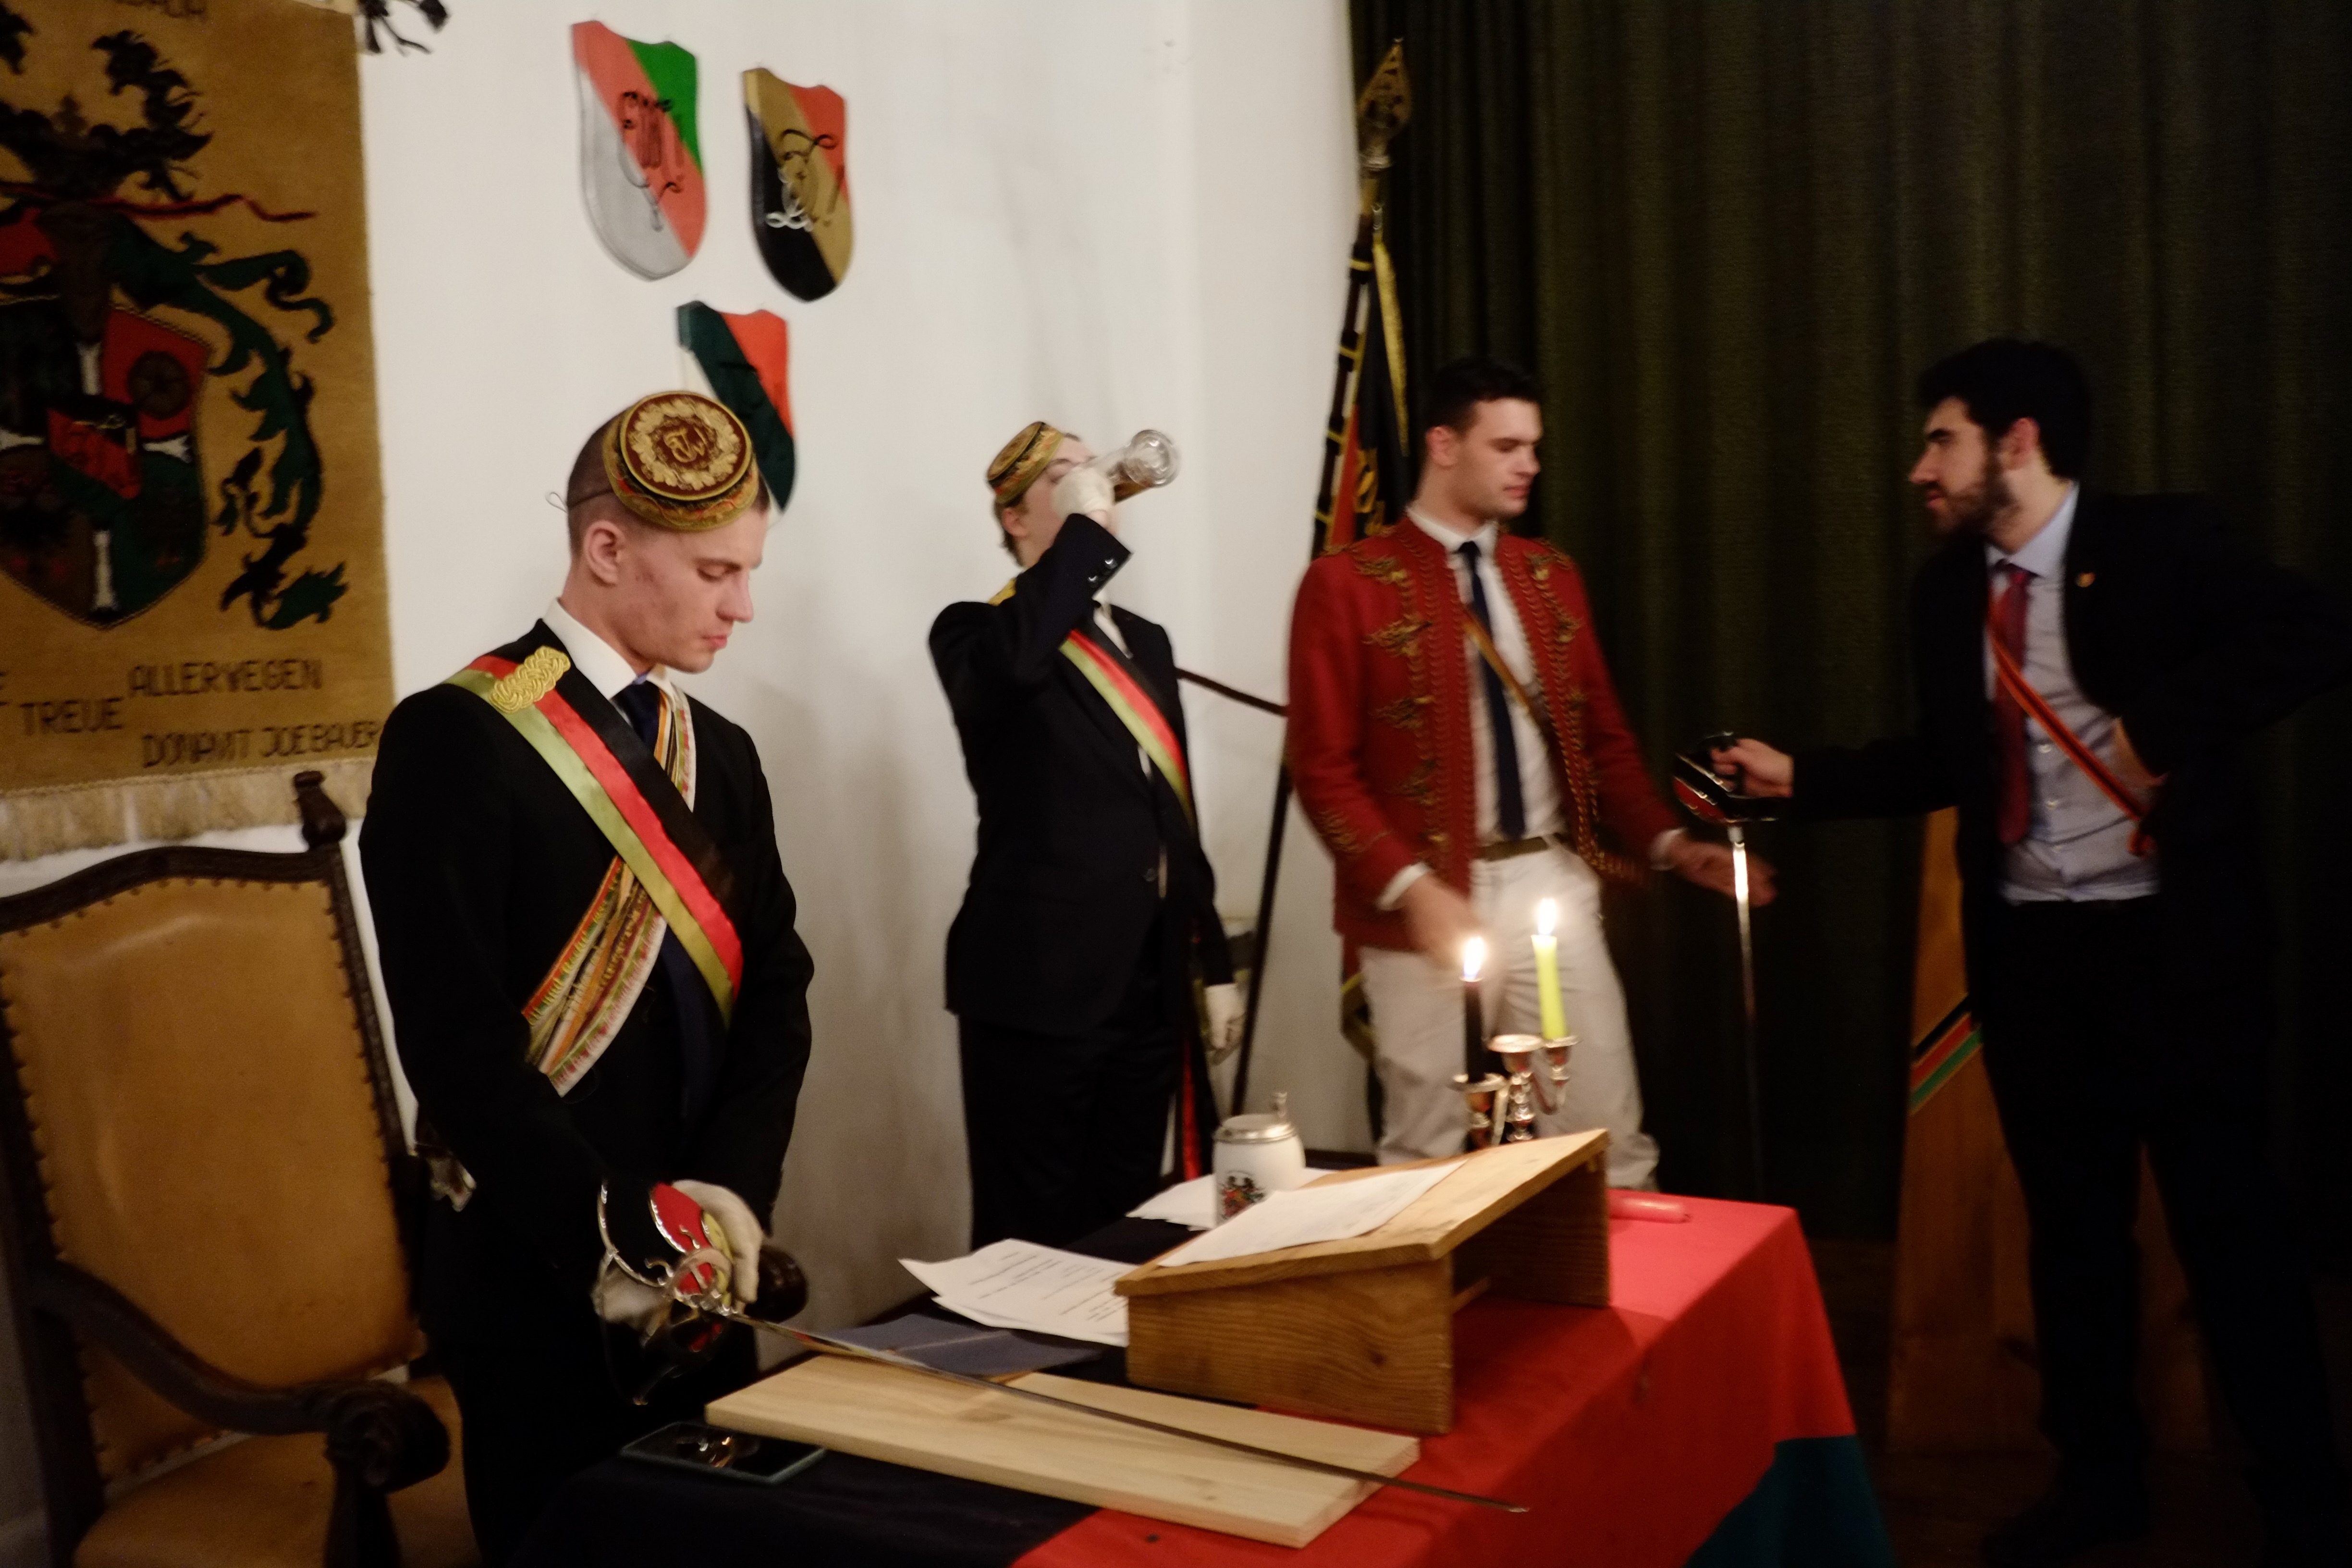
\includegraphics[width=.8\linewidth]{./Bilder/Oelympische Spiele/DSCF6082.jpeg} 
		\caption{Bei der Abkneipe des WS 2023/24\\Von links nach rechts:\\ Senior des SS 2024 Benjamin Buhl \\Fuxmajor Antoine Leyder\\Leiter der Oelympischen Spiele Fabian Heinrich, \\Fux Mathias Brezina (ausgetreten)\\
		} 
	\end{center}
\end{figurehere}

%
%\begin{figurehere}
%	\begin{center}
%		\includegraphics[width=.8\linewidth]{Bilder/pios2}
%		\caption{Realer Aufbau} 
%	\end{center}
%\end{figurehere}
\newpage

\section{100-Semester-Bandverleihung}
\sectionmark{100-Semester-Bandverleihung}

\begin{multicols}{2}
Am 22. März 2024 machten sich Bbr. Philipp Kopystynski und der Verfasser
dieser Zeilen auf nach Vilshofen, um Bbr. Pfarrer Gotthard Weiß sein
längst überfälliges 100-Semesterband zu überreichen. Dies war notwendig,
da der Jubilar gesundheidsbedingt leider nicht mehr nach München reisen
kann. Der Phil-X hat mich dazu dankenswerterweise autorisiert.
Bbr. Weiß wurde am 10. März 1952 geboren und trat nach dem Abitur
unserer lieben Vandalia bei. Die feierliche Reception erfolgte am 17.
November 1971. Geburscht wurde Bbr. Gotthard am 23. Juni 1972. Er
studierte Mathematik für das Lehramt und schloss dieses Studium auch
erfolgreich ab. Doch dann vernahm er den Ruf unseres Herrn und er ging
in seine Heimatdiozöse Passau und nahm das Studium der Theologie auf. In
diesem Zusammenhang war er auch der Gründungssenior der KdStV
Oeno-Danubia zu Passau im CV.
Bbr. Gotthard war vorher auch recht aktiv in der Va: XXXX im WS 72/73, X
im SS 74, FM im WS 74/75. Legendär ist für mich der Mut in das Programm
zu drucken, dass auf dem Haus der Sieg der deutschen
Fussballnationalmannschascht angeschaut und anschließend gefeiert wird.
Ich hätte mich das bei meinen beiden Senioraten nicht getraut. Aber er
hat Recht behalten!
Später gab es tolle Einladungen zu Geburtstagen oder Priesterjubiläen
in  ein jeweils eigens für ihn aufgestelltes Bierzelt. Danke Gotthard,
diese Tage werde ich nie vergessen.
Zwei Jahrzehnte hielt Bbr. Gotthard im Advent Messen in den
Verbindungsräumen der Vandalia. Ich war immer da - in der Regel waren
wir vorher in der Stadt - und werde auch dies nicht vergessen. Aber
daneben ist er auch immer als Seelsorger und Beichtvater für
Bundesbrüder tätig. Es gab jede Menge Aktiven- bzw. Fuxenfahrten zu ihm,
denn er kann auch Bundesbrüder begeistern, die nicht jeden Sonntag in
die Kiche gehen.
Bbr. Gotthard hatte zwei Confüxe, die leider schon verstorben sind:
Norbert Wartha - mein Zipfbruder und Festredner als ich X der Va war -
(2000) und Wilfried Schneider (2023). Lasst uns an sie denken!
Der Tag mit Bbr. Gotthard war sehr schön. Wir sind nach einem
Bergrüßungsbier für mich zu einem schönen Landgasthof in der Nähe
gefahren. Dort fand dann erst die Bandübergabe statt. Der Jubilar
bestand auf einen ordentlichen Streifen aus dem Glas. Dem sind wir
natürlich gerne nachgekommen. Der Wirt wurde vorgewarnt: Wir haben die
Vandalenstrophe geschmettert. Ein anderer Gast hat sogar applaudiert.
Zum Schluss hatt Bbr. Gotthard mir noch seinen Va-Krug mit seinem
Biernamen \glqq Springerl\grqq ~ überreicht, damit ich ihn in der Va an einen
exponierten Platz stelle. Das mache ich natürlich gerne!
Hoffen wir auf viele weitere Bundesbrüder, die unserer Vandalia 50
Jahre, 100 Semester, treu bleiben, damit wir noch viele solche Bänder
verleihen können.
Vivat, crescat, floreat Vandalia ad multos annos!

	\begin{flushright}
		\hfill\emph{Dr. Thomas Strieder AlgA!, Va!, Elb!}
	\end{flushright}
	%	

\end{multicols}

\begin{center}
\begin{figurehere}
		
\includegraphics[width=.55\linewidth]{./Bilder/1.4.100Semesterband/2.bild.png} 
\end{figurehere}

\begin{figurehere}
  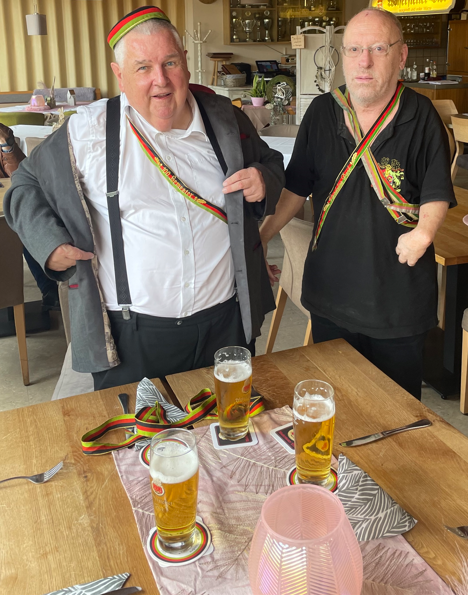
\includegraphics[width=.55\linewidth]{./Bilder/1.4.100Semesterband/1.bild.png} 
  \captionsetup{justification=centering,margin=2cm}
  \caption{Feierliche Bandverleihung an Gotthard Weiß Va! (links) durch\\ ~Dr. Thomas Strieder AlgA! Va! Elb! (rechts)}
\end{figurehere}
\end{center}


%
%\begin{figurehere}
%	\begin{center}
%		\includegraphics[width=.8\linewidth]{Bilder/pios2}
%		\caption{Realer Aufbau} 
%	\end{center}
%\end{figurehere}
\newpage

\section{Back to the roots: \\ ~~Aktivenfahrt in unsere Gründungsstadt Prag}
\sectionmark{Aktivenfahrt nach Prag}

\begin{multicols}{2}
Liebe Bundesbrüder,
habt Ihr Euch schon mal gefragt, was wohl aus den legendären Pragfahrten der Vandalia geworden ist? Nun der alte Vandalen-Geist lebt weiter! Im Folgenden ein kleiner Bericht über unsere jüngste Exkursion vom 30.05.- 02.06.2024 in die goldene Stadt.\\

\textbf{Donnerstag, 30.05.2024}\\
Nach der Fonleichnamsprozession am Vormittag konnte die Anreise für insgesamt neun Vandalen mit dem Zug ALX am Nachmittag gegen halb fünf in unsere Gründungsstadt beginnen. Die Stimmung war schon zu Beginn im Abteil ausgelassen, Bier floß in adäquaten Maßen und erste Lieder erklangen. Da es zu diesem Zeitpunkt keine direkte Verbindung nach Prag gab, mussten wir am Abend in Domazlice umsteigen. Der Umstieg bereitete keine Probleme, da wir uns schon auf tschechischen Terrain befanden und somit von der Deutschen Bahn und ihrer regelmäßigen Unzumutbarkeit erlöst wurden. Dort stieß auch der Cartellbruder Oskar unserer Patentochter KDStV Oeno-Danubia Passau hinzu, der uns die weiteren Tage in Prag begleitete und als gebürtiger Tscheche unsere Gründungsstadt näher beleuchtete. Pünktlich und reichlich gut gelaunt aufgrund des reibungslosen Ablaufs bisher erreichten wir Prag gegen halb elf am Abend. Nachdem unser Consenior Joey erklärte welche Tickets für den ÖPNV wir am besten erwerben sollten, konnten wir uns auf dem Weg zu unserem Quartier machen, welches von erwähntem Cartellbruder der Oeno-Danubia dankenswerter Weise zur Verfügung gestellt wurde. Als wir uns in der großzügigen Wohnung eingerichtet hatten, galt es anschließend noch eine Kleinigkeit zu sich zu nehmen und die nahegelegenen Kneipen zu inspizieren. Jedoch ging der Abend nicht allzu lang, denn es stand einiges an Programm am nächsten Tage an.\\
\\
\textbf{Freitag, 31.05.2024}\\
Nach einem ausgiebigen Frühstück (Katerfrühstück für so manchen Bundesbruder) in der Nähe von Svetozor stand Kultur auf dem Programm. Wir besichtigten zunächst den allseits bekannten Prager Schipkapass. Endlich angekommen und mit ausreichend Wegbier ausgestattet, konnte sich jeder Bundesbruder sehr gut vorstellen, wie es wohl zu alten Zeiten dort lustig zugegangen ist. Eine Kneipe zu schlagen war nicht möglich, aber wir ließen es uns nicht nehmen, unsere Farbenstrophen zum Besten zu geben. Leider machte uns das Wetter bald einen Strich durch die Rechnung. Als nach einiger Zeit ein Wolkenbruch über uns hineinbrach, beschloßen wir den Rückweg anzutreten, obwohl einige Bundesbrüder sicherlich noch gerne mehr Zeit an dem zu seiner Zeit legendären Verbindungslokal verbracht hätten. Wir versuchten anschließend unser Glück durch den Prager Bierzoo. Dieser meint nichts anderes als die besten, preiswertesten, urigsten Kneipen Prags. Unglücklicherweise ließ der Regen keinesfalls nach und so waren wir selbstverständlich nicht die einzigen, die Unterschlupf in einer urigen Kneipe suchten. Nach mehreren vergeblichen Versuchen, fanden wir zumindest eine Kneipe, in der wir uns bei einem Glas feinstem Pilsener Urquell vom Regen regenerieren konnten. Als der Regen nachließ, gaben uns unser Consenior Joey und Cartellbruder Oskar eine kleine Stadtführung. Dabei durfte selbstverständlich ein Gang über die Karlsbrücke mit dem heiligen Nepomuk nicht fehlen. Des Weiteren machten wir einen Halt am Ort unser alten Wirkungsstätte in der Smetschkagasse 22. Von außen betrachtet ein ordinäres Wohnhaus, konnte man sich kaum vorstellen, dass dort einmal unsere Mutterverbindung Ferdinandea, unsere Tochterverbindung Saxo-Bavaria und wir unsere
Kneipen schlugen. Ferner war ein Besuch der Prager Burg unerläßlich. Mittlerweile war das Wetter kein Störfaktor mehr und so konnten wir dort den herrlichen Ausblick über Prag genießen. Nach einem vorzüglichen Abendessen statteten wir der bekannten Bar THE PUB in der Prager Neustadt einen Besuch ab. THE PUB ist eine Barkette, die dafür berüchtigt ist, dass jeder Tisch mit seinen eigenen Zapfhahn ausgestattet ist. Zudem gibt es am Tisch eine Anzeige mit mehreren Bierkonten, sodass man sieht, wie viel man gerade gezapft hat. Der große Vorteil besteht darin, dass man nie auf die Bedienung bzw. sein nächstes Bier zu warten hat, sondern direkt selbst zapfen kann, sobald man leergezogen hat. Wohl überlegt hatte unser Consenior Joey vorab schon reserviert, denn die Bar war wie erwartet überaus voll und anderenfalls nicht besuchbar. Dort machten wir wenig überraschend Bekanntschaft mit anderen Deutschen, einer Fußballmannschaft. Etwas enttäuschend konnten wir gesanglich mit unseren Landsleuten nicht mithalten, jedoch war das nach einigen Gläsern Pilsener Urquell schon wieder vergessen und jeder Vandale war am Ende doch zufrieden. Im Hinblick auf das nächste Highlight am folgenden Tag, die Fahrt nach Pilsen zur Brauereiführung, übertrieben wir es auch nicht und der Abend fand kein allzu langes Ende. Vandalen können tatsächlich auch vernünftig sein.\\
\\
\textbf{Samstag, 01.06.2024}\\
Ein weiterer Höhepunkt war am Samstag die Fahrt nach Pilsen. Gegen zwei Uhr nachmittags angekommen, hatte unser Consenior Joey im Lokal Pod Divadlem unweit der Brauerei reserviert. Sicherlich war es keine schlechte Idee sich vor der Brauereiführung noch etwas Reichhaltiges zu genehmigen. So fiel bei den meisten die Wahl auf Schweinshaxe oder Schnitzel. Ausreichend gestärkt konnte nun die Brauereiführung mit Verköstigung um drei Uhr beginnen.
Wir erfuhren, dass Pilsner Urquell als Lagerbier seit 1842 in Pilsen gebraut wird und als das erste Pilsner Bier der Welt gilt. Es wurde ursprünglich von dem bayerischen Braumeister Josef Groll entwickelt. Seine helle Farbe und der einzigartige Geschmack revolutionierten die Bierwelt und machten Pilsner Urquell zum Vorbild für viele andere Biersorten. Man erkennt sofort, wie stolz die Brauerei auf ihre Tradition ist und dass sie das Bier nach wie vor nach Originalrezeptur braut. Jedoch bekommt man nur in der Brauerei das Pilsner Urquell in Originalrezeptur unfiltriert und unpasteurisiert. Davon konnten wir uns selbst überzeugen, als wir uns im Bierstüberl der Brauerei mehrere Gläser des Originalen Pilsner Urquells genehmigten und einen Unterschied zum Pilsener Urquell feststellten, welches in Bars, Kneipen, Supermärkten etc. angeboten wird. Leider konnte man keine Kostproben des Originals in der Brauerei erwerben, um sie nach München mitzunehmen. Deshalb nutzen wir die verbliebene Zeit umso mehr, um uns das Original Pilsner Urquell schmecken zu lassen.
Trotz des reichlichen Biergenusses erwischten alle Vandalen pünktlich den Zug für die Rückfahrt nach Prag um sieben Uhr abends. Angekommen um halb neun in Prag, machten wir uns in verschiedenen Gruppen auf, das Prager Nachtleben ein letztes Mal zu genießen. Die Nacht war für die einzelnen Bundesbrüder unterschiedlich lang und die Taxifahrt zurück zu unserem Quartier unterschiedlich teuer, jedoch kamen alle Bundesbrüder insgesamt auf ihre Kosten, was den Unterhaltungswert anging.\\

\textbf{Sonntag, 02.06.2024}\\
Um halb zwölf mittags traten wir naiv die Heimreise gen München an. Gott sei Dank hatte der Consenior wieder zwei Abteile reserviert. Der Zug zurück war brechend voll und wir mussten
uns erstmal zu unseren reservierten Plätzen durchkämpfen und letztlich die Leute, die auf unseren Sitzen schon saßen, bitten, Platz zu machen. Erschöpft aber auch freudig gestimmt durch die vergangenen Tage, wurde uns auf der Rückfahrt mit der Zeit bewußt, wie viel es eigentlich in Süddeutschland geregnet hatte, als wir durch die Oberpfalz fuhren. Kurz vor Weiden wurde dann durchgesagt, dass der Zug nur bis Regensburg fahre und es bis auf Weiteres keine Verbindung nach München gäbe. Ein Bundesbruder stieg daraufhin in Weiden aus und ließ sich von seinen Eltern abholen, die in der Nähe wohnen. Der Rest fuhr erstmal weiter bis nach Regensburg. Nach kurzer Absprache boten uns freundlicherweise die Cartellbrüder der KDStV Rupertia Regensburg Unterkunft bis zum nächsten Tag an, was jedoch nur von drei Vandalen in Anspruch genommen wurde. Die übrigen Vandalen versuchten ihr Glück, indem sie mit dem Zug über Landshut fuhren oder den Flixbus nahmen. Trotz des Hochwassers in Regensburg, schafften es am Ende alle Vandalen unbeschadet in München anzukommen, sei es am späten Sonntagabend oder frühen Montagmittag gewesen.
Insgesamt kann man mal sagen, dass die Aktivenfahrt nach Prag abermals ein voller Erfolg war! Sehr empfehlenswert ist für weitere Fahrten in unsere Gründungsstadt der Besuch des Schipkapasses und die Fahrt nach Pilsen zur Brauereiführung des Originalen Pilsener Urquells. Ein besonderer Dank gilt an dieser Stelle unserem Consenior Joey Jurcik, der alles vorzüglich geplant hatte, sodass die Fahrt reibungslos stattfinden konnte. Ein weiterer Dank gilt dem Cartellbruder der Oeno-Danubia Oskar Stejfa, der uns seine Wohnung als Unterkunft zur Verfügung stellte und ebenfalls wie Joey durch die Stadt führte und die Geheimtipps der Stadt zeigte, die ein gewöhnlicher Tourist nie kennen würde. Danke an die zwei Organisatoren, die trotz einiger \glqq Herausforderungen\grqq ~ alles im Griff hatten.
In diesem Sinne, auf die nächste Fahrt!\\
Vivat, crescat, floreat Vandalia ad multos annos!

\end{multicols}

\begin{flushright}
		\hfill\emph{Philipp Kopystynski v/o Rammbock Va!\\ Raphael Frank Va!}
	\end{flushright}
	%	
			

	

%
%\begin{figurehere}
%	\begin{center}
%		\includegraphics[width=.8\linewidth]{Bilder/pios2}
%		\caption{Realer Aufbau} 
%	\end{center}
%\end{figurehere}
\newpage

\section{Bilder Aktivenfahrt Prag SS 2024}
\sectionmark{Bilder Aktivenfahrt Prag SS 2024}

%\begin{figurehere}
%	\begin{center}
%		\includegraphics[width=\linewidth]{Bilder/andechs2.jpg}
%%		\caption{xxx} 
%	\end{center}
%\end{figurehere}
	
\begin{center}
\begin{figurehere}
  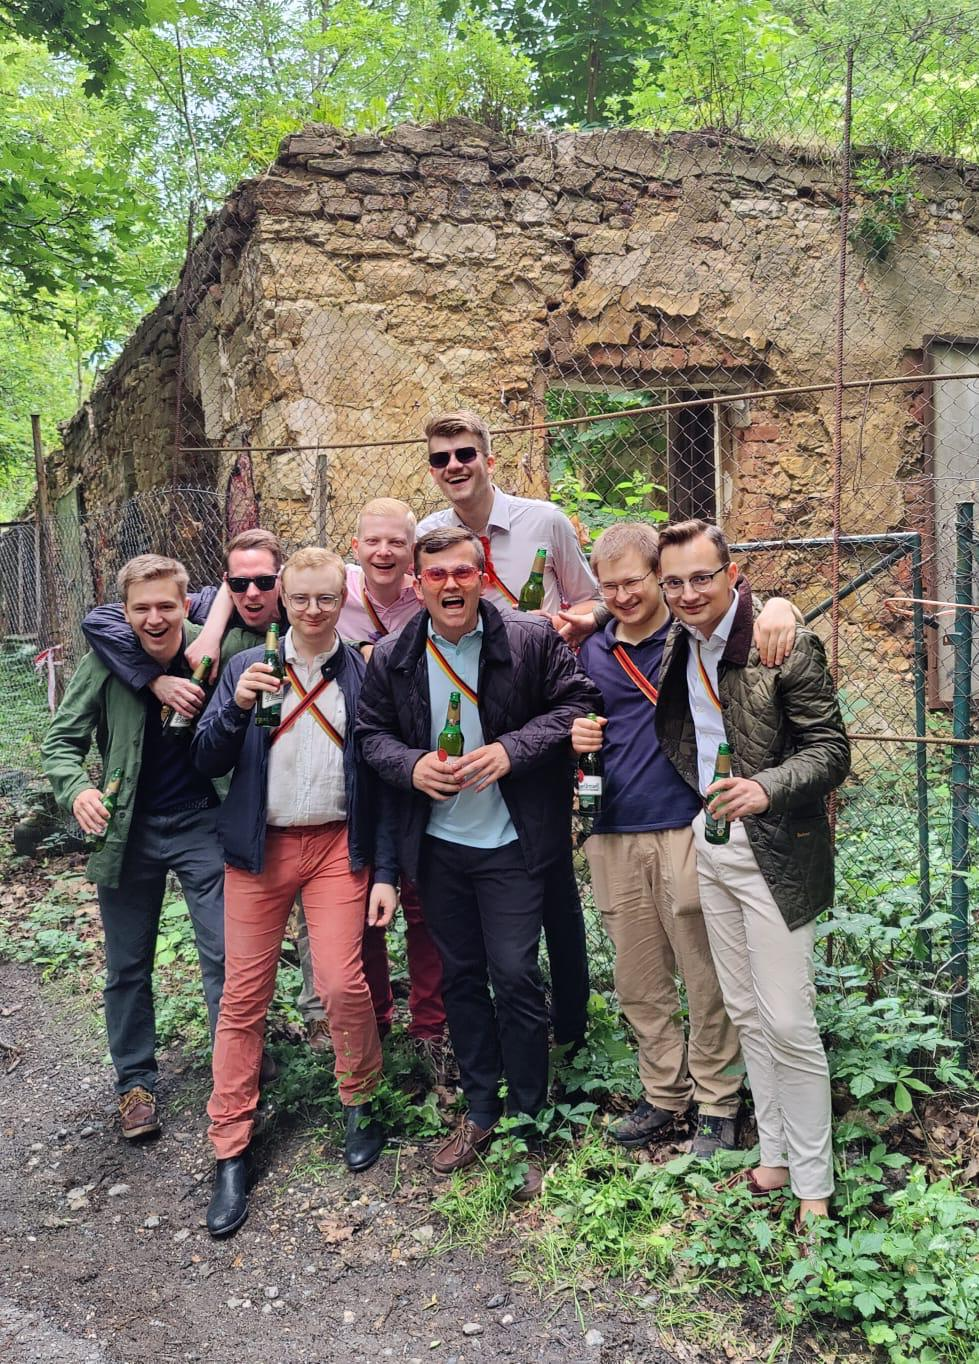
\includegraphics[width=.7\linewidth]{./Bilder/1.5BackToTheRootsAktivenfahrtPrag/1.bild.jpeg} 
        \caption{Vandalen am legendären Schipkapass}
\end{figurehere}
\end{center}	
	

\begin{center}
\begin{figurehere}
  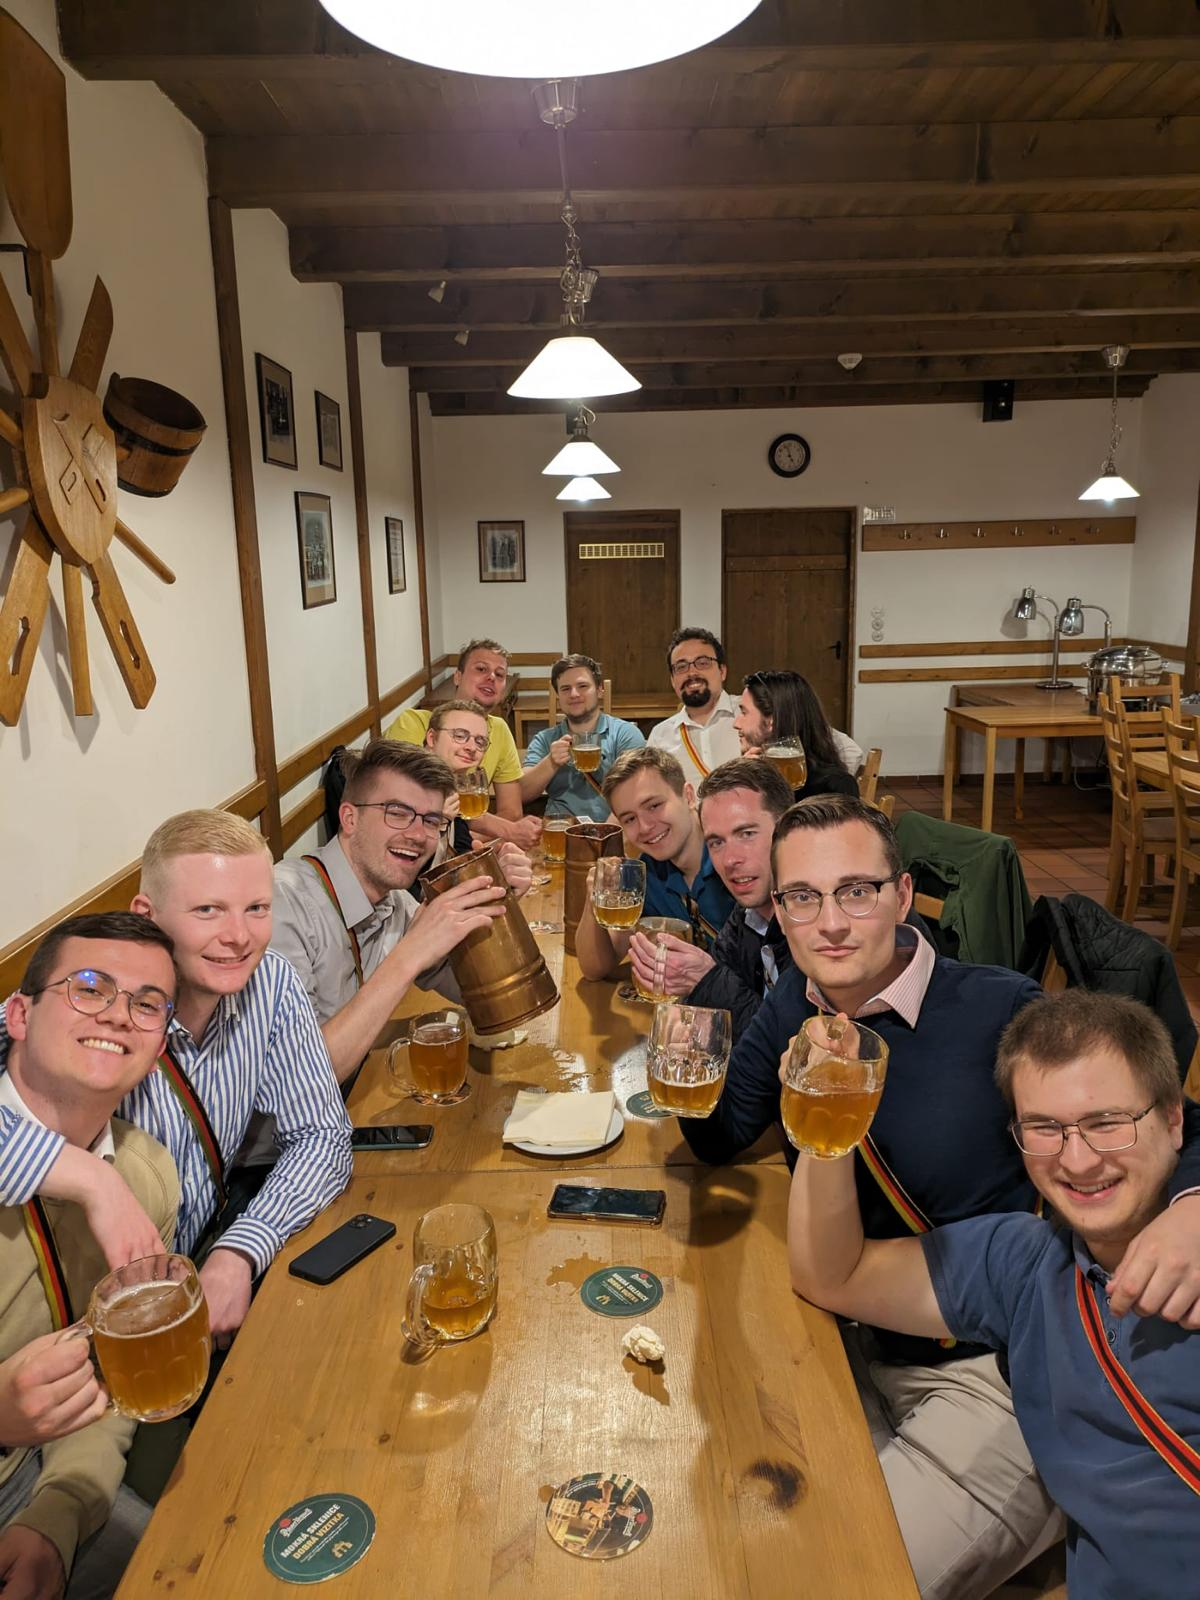
\includegraphics[width=.7\linewidth]{./Bilder/1.5BackToTheRootsAktivenfahrtPrag/2.bild.jpeg} 
  \caption{Verköstigung des Originalen Pilsener Urquells im Bierstüberl}
\end{figurehere}
\end{center}

	\newpage

\begin{center}
\begin{figurehere}
  
\includegraphics[width=.7\linewidth]{./Bilder/1.5BackToTheRootsAktivenfahrtPrag/3.bild.jpeg} 
  \caption{Adäquate Stoffversorgung für die Zugfahrt}
\end{figurehere}
\end{center}

\begin{center}
\begin{figurehere}

\includegraphics[width=.7\linewidth]{./Bilder/1.5BackToTheRootsAktivenfahrtPrag/4.bild.jpeg} 
  \caption{Ausgewogenes (Kater)frühstück am Morgen}
\end{figurehere}
\end{center}	

\begin{center}
\begin{figurehere}

\includegraphics[width=.7\linewidth]{./Bilder/1.5BackToTheRootsAktivenfahrtPrag/5.bild.jpeg} 
  \caption{Selbstgezapftes Bier in THE PUB}
\end{figurehere}
\end{center}

\begin{center}
\begin{figurehere}
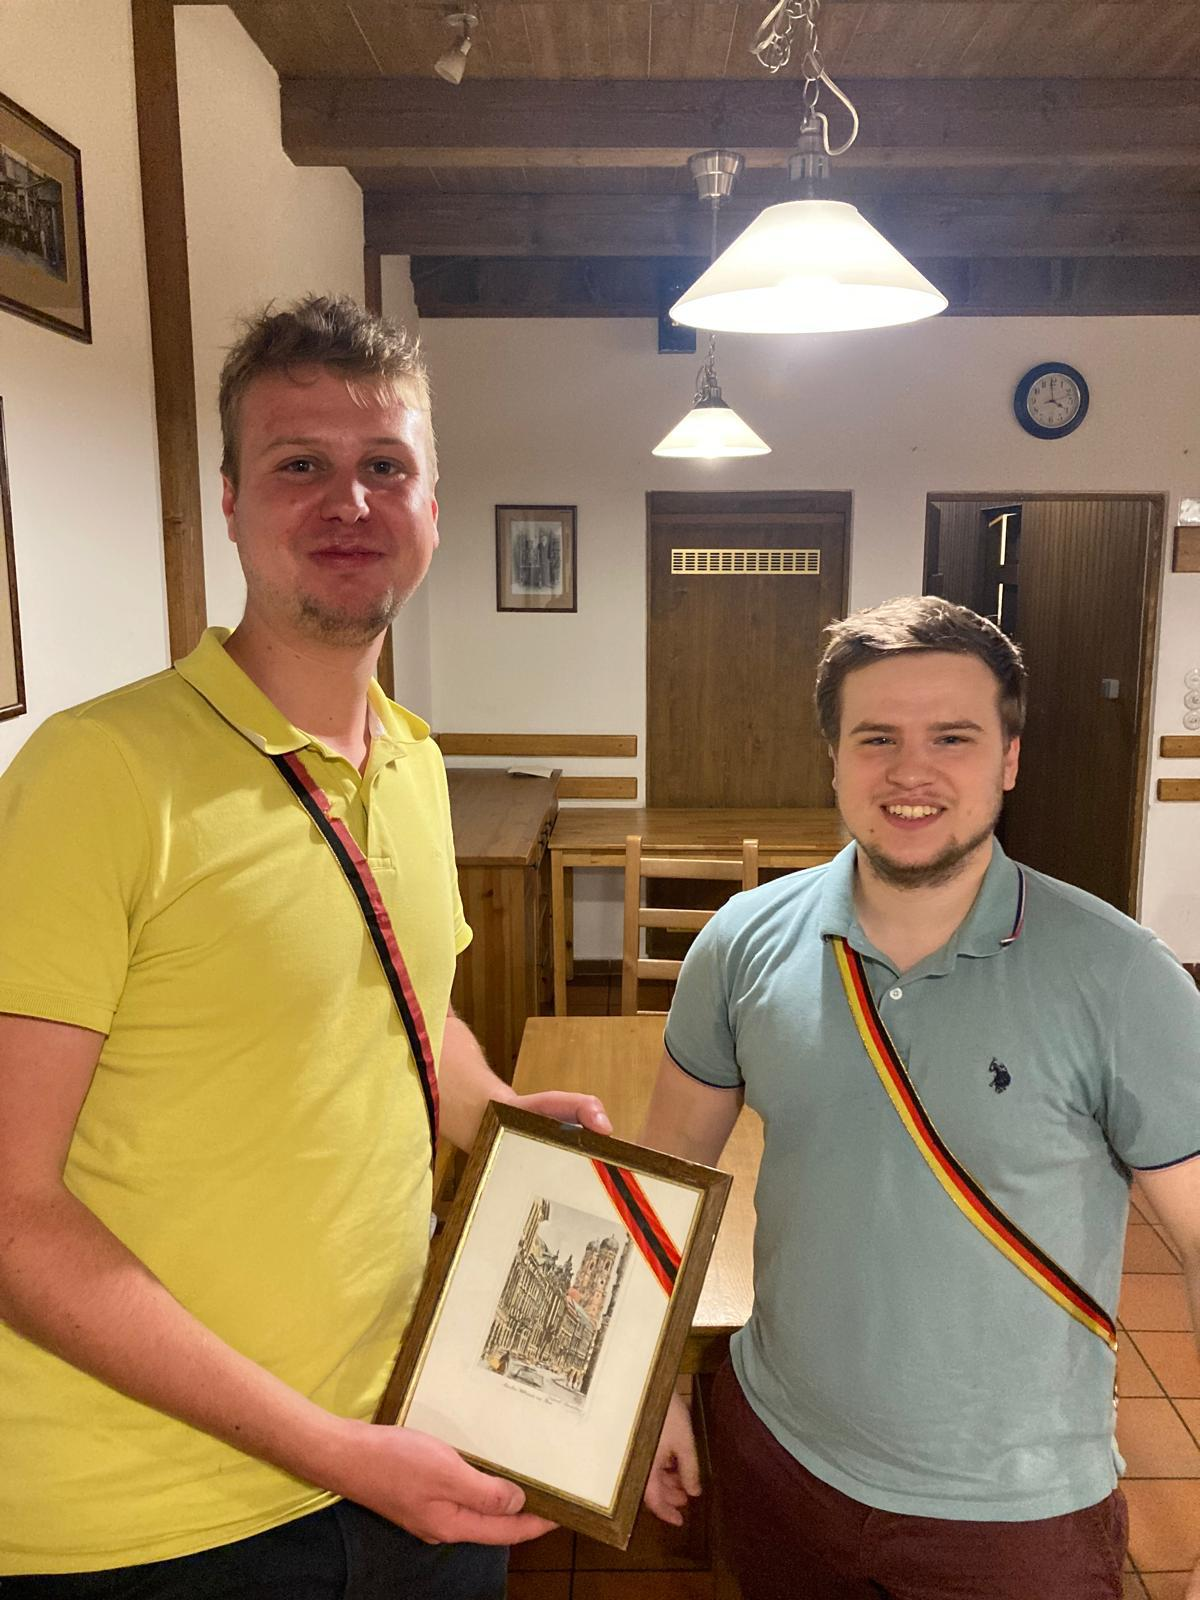
\includegraphics[width=.7\linewidth]{./Bilder/1.5BackToTheRootsAktivenfahrtPrag/6.bild.jpeg} 
  \caption{Der Consenior Joey (rechts) überreicht unser Gastgeschenk an den ortskundigen Cartellbruder der Oeno-Danubia Passau Oskar (links)}
\end{figurehere}
\end{center}

\begin{center}
\begin{figurehere}
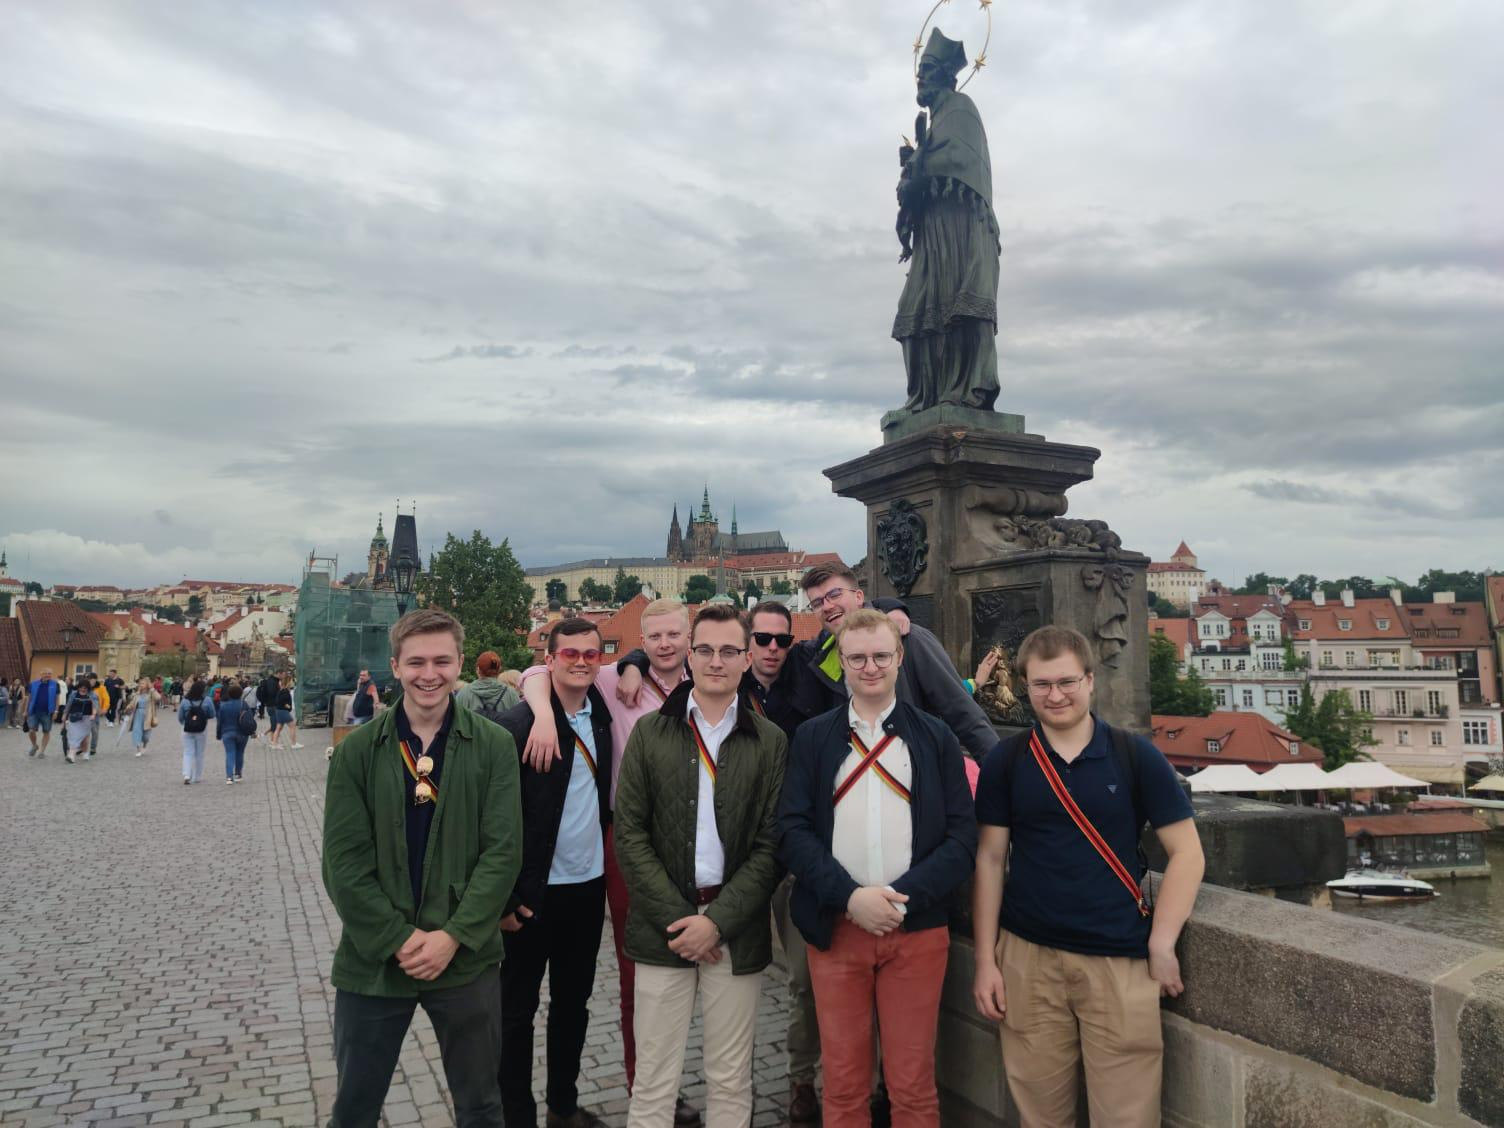
\includegraphics[width=.7\linewidth]{./Bilder/1.5BackToTheRootsAktivenfahrtPrag/7.bild.jpeg} 
  \caption{Vandalen auf der Karlsbrücke vor dem Heiligen Nepomuk}
\end{figurehere}
\end{center}

%
%\begin{figurehere}
%	\begin{center}
%		\includegraphics[width=.8\linewidth]{Bilder/pios2}
%		\caption{Realer Aufbau} 
%	\end{center}
%\end{figurehere}
\newpage

\section{Leben aus Stickstoff – die Zukunft der Ammoniakproduktion}
\sectionmark{N2-Reduktion}

%\begin{figurehere}
%	\begin{center}
%		\includegraphics[width=\linewidth]{Bilder/andechs2.jpg}
%%		\caption{xxx} 
%	\end{center}
%\end{figurehere}

\begin{multicols}{2}	
Das Stickstoff-Atom ist einer der Grundbausteine lebendiger Materie. Mikroorganismen fixieren den in molekularer Form (N2) vorliegenden Luftstickstoff und machen ihn nutzbar für die Bildung von Proteinen und anderen Biomolekülen. Wie auch für Sauerstoff oder Kohlendioxid hat sich im Zuge der Entwicklung des Lebens ein komplexer Stickstoff-Kreislauf auf der Erde ausgebildet. Spätestens seit der Entwicklung des Haber-Bosch-Verfahrens zu Beginn des 19. Jahrhunderts greift die Menschheit in industriellem Maßstab in diesen Kreislauf ein. Zur Ernährung der wachsenden Weltbevölkerung wird in gigantischen Mengen Ammoniak (NH3) synthetisiert, der als Ausgangsstoff für pflanzlichen Dünger dient. Durch die Reaktivität des Ammoniak-Moleküls wird der darin enthaltene Stickstoff für organische Synthesen nutzbar – anders als im molekularen Stickstoff, dessen energetisch günstige Dreifachbindung extrem stabil und schwer aufzuspalten ist. Die energetisch aufwendige Fixierung des Luftstickstoffs wird der Natur damit gewissermaßen abgenommen, und Nutzpflanzen können schneller und dichter wachsen, als die natürliche Bodenverfügbarkeit von fixiertem Stickstoff es erlauben würde. Dies ist seit dem 20. Jahrhundert eine notwendige Voraussetzung für die Ernährung der rasant gewachsenen Weltbevölkerung.
\\
Über die Risiken, die mit der massiven Beeinflussung des globalen Stickstoffkreislaufes einhergehen, ist in der breiten Gesellschaft kaum etwas bekannt – die Verankerung entsprechender Forschungsergebnisse im kollektiven Denken und Handeln erleben wir gerade erst im Bezug auf anthropogene CO2- und Treibhausgas-Emissionen. Doch auch hier schon spielt die globalen Ammoniak-Produktion, bedingt durch ihre enormen Ausmaße, eine elementare Rolle. Die Herstellung der jährlich verbrauchten über 100 Megatonnen Ammoniak beansprucht 2\% der gesamten weltweiten Energieproduktion und verbraucht 3-5\% der jährlich geförderten Erdgasmenge. Damit einher geht ein signifikanter Beitrag zu den globalen CO2-Emissionen, und damit zum menschengemachten Klimawandel. Wer sich davon nicht behelligen lässt, ist vielleicht für ein geopolitisches Argument empfänglicher: Das bislang alternativlose Haber-Bosch-Verfahren zur industriellen Ammoniak-Herstellung ist wegen der erforderlichen hohen Temperaturen und Drücke nur in großtechnischen Anlagen wirtschaftlich realisierbar. Die Zentralisierung der Produktion, inklusive einer darauf ausgerichteten Infrastruktur, hat heutzutage ein globales Ausmaß. 30\% der globalen Ammoniak-Produktion erfolgen in China, danach kommen mit je 8-10\% die USA, die EU, Indien, Russland und der nahe Osten. Da die Produktion auf Erdgas angewiesen ist, ist dessen billige Verfügbarkeit eine Voraussetzung. Damit kann der Export von Ammoniak und abgeleiteten Produkten nur allzu leicht ein Spielball geopolitischer Interessen werden.
\\
Die Chancen alternativer Herstellungsverfahren liegen nun auf der Hand. Eine dezentrale Produktion ohne Abhängigkeit von Erdgas könnte, großflächig umgesetzt, die Energiewende unterstützen und die Souveränität von Verbraucherländern stärken. Dazu kommen bei einer verbrauchernahen Erzeugung die eingesparten Emissionen, die durch den weltweiten Transport anfallen. Welche Möglichkeiten gibt es? Für die nächsten 20 bis 30 Jahre wird ein „grünes“ Haber-Bosch-Verfahren die größte industrielle Bedeutung haben, bei dem der notwendige Wasserstoff durch Elektrolyse (mit Strom aus erneuerbaren Quellen) statt durch die Verarbeitung von Erdgas bereitgestellt wird. Für die Zeit danach werden mehrere, bislang leider nicht skalierbare Lösungen erforscht. Von der Natur inspirierte künstliche Enzyme, lithiumhaltige Elektrolytlösungen, durch Sonneneinstrahlung beheizte Reaktoren – das Spielfeld ist weit. Fest steht, dass eine neue Art der Ammoniaksynthese unsere Gesellschaft und unsere Wirtschaft prägen wird, ebenso, wie es der Haber-Bosch-Prozess die letzten hundert Jahre getan hat.
\\
Zum Schluss ein paar Worte zu meiner Verbindung mit diesem Thema: Im Rahmen meiner Doktorarbeit am Walter-Schottky-Institut der Technischen Universität München erforsche ich Halbleitermaterialien, die wie Solarzellen Energie in Form von angeregten Elektronen bereitstellen können. Ich versuche, mit diesen Elektronen die Reduktion von Stickstoff zu Ammoniak in Wasser anzutreiben. Würde dieser Ansatz funktionieren, böte er eine gut skalierbare Lösung, ähnlich wie die Brennstoffzelle zur Wasserstofferzeugung. Momentan tragen unsere Bemühungen keinen Erfolg, aber ich bin gespannt, was die nächsten 3 Jahre noch bringen werden. Über dieses Thema gibt es noch vieles zu berichten, und gerne empfehle ich weiterführende Artikel.
\\
Die Geschichte des Haber-Bosch-Prozesses und der namensgebenden Wissenschaftler ist mit ihren vielen historischen Verflechtungen und ihrer moralischen Ambivalenz eine unbedingte Empfehlung zur persönlichen Weiterbildung. Die künstliche Ammoniaksynthese brachte im ersten Jahrhundert ihrer Erfindung Leben und Tod für Hunderte Millionen von Menschen. Wir dürfen hoffen, dass sie im folgenden Jahrhundert ein beispielhafter Erfolg auf dem Weg der ökologischen und wirtschaftlichen Transformation unserer Gesellschaft wird.
\\
\begin{flushright}
		\hfill\emph{Maximilian Christis Va!}
	\end{flushright}
		
\end{multicols}


\begin{figurehere}
	\begin{center}
		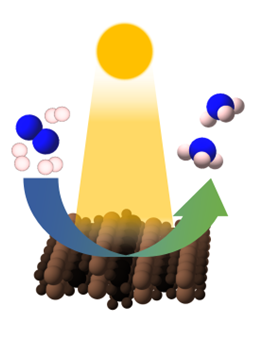
\includegraphics[width=.4\linewidth]{./Bilder/2.0.Stickstoff_Reduktion/Bild1.png} \caption{Prozess der photochemischen Ammoniak-Synthese an der Oberfläche eines Katalysators.} 
	\end{center}
\end{figurehere}



\begin{figurehere}
	\begin{center}
		 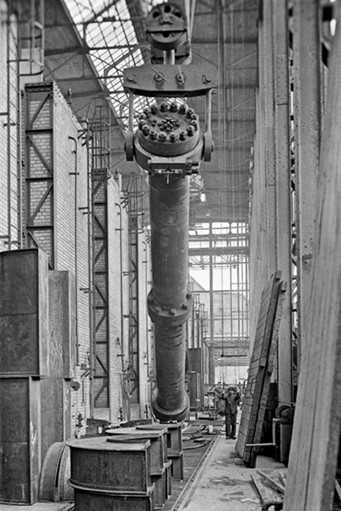
\includegraphics[width=.4\linewidth]{./Bilder/2.0.Stickstoff_Reduktion/Bild2.jpg} 
		 \caption{Erster Haber-Bosch-Reaktor im BASF-Werk Oppau, 1913. © BASF}
	\end{center}
\end{figurehere}


%
%\begin{figurehere}
%	\begin{center}
%		\includegraphics[width=.8\linewidth]{Bilder/pios2}
%		\caption{Realer Aufbau} 
%	\end{center}
%\end{figurehere}
\newpage

\section{Genesis 2: Eine theologische Abhandlung}

\sectionmark{Gebein von meinem Gebein und \newline Fleisch von meinem Fleisch}

\begin{center}
\textit{\color{gray}Die Erschaffung der Frau in Genesis 2,18-25}
\end{center}

In den aktuellen Debatten der Gesellschaft spielt die Frage der Gerechtigkeit im Verhältnis der Geschlechter eine große Rolle. Oft wird dem Alten Testament vorgeworfen, die Frau abzuwerten und dabei wird nicht selten Gen 2,18-25 als Beispiel angeführt. Ob es dem Text gerecht wird, wollen wird uns nun anschauen.

\begin{multicols}{2}
\textbf{Text 18:}\\ \textit{Und der HERR, Gott, sprach: Es ist nicht gut, dass der Mensch allein ist; ich will ihm eine Hilfe machen, die ihm entspricht. 19 Und der HERR, Gott, bildete aus dem Erd- boden alle Tiere des Feldes und alle Vögel des Himmels, und er brachte sie zu dem Menschen, um zu sehen, wie er sie nennen würde; und ge- nau so, wie der Mensch sie, die lebenden We- sen, nennen würde, ⟨so⟩ sollte ihr Name sein. 20 Und der Mensch gab Namen allem Vieh und den Vögeln des Himmels und allen Tieren des Feldes. Aber für Adam [für ihn als Mensch] fand er keine Hilfe, ihm entsprechend. 21 Da ließ der HERR, Gott, einen tiefen Schlaf auf den Menschen fallen, sodass er einschlief. Und
 nahm eine von seinen Rippen und verschloss ihre Stelle mit Fleisch; 22 und der HERR, Gott, baute die Rippe, die er von dem Menschen ge- nommen hatte, zu einer Frau, und er brachte sie zum Menschen. 23 Da sagte der Mensch: Diese endlich ist Gebein von meinem Gebein und Fleisch von meinem Fleisch; diese soll Männin heißen, denn vom Mann ist sie genommen. 24 Darum wird ein Mann seinen Vater und seine Mutter verlassen und seiner Frau anhängen, und sie werden zu einem Fleisch werden. 25 Und sie waren beide nackt, der Mensch und seine Frau, und sie schämten sich nicht. (Elberfelder Bibel, Gen 2,18-25)}
\end{multicols}

Bevor wir uns der Analyse des Textes widmen, müssen wir einen kurzen Blick auf die Geschichte des Textes werfen. Die Entstehung des Pentateuchs (und des Buches Genesis als Teil des Pentateuchs) ist sehr komplex und vielschichtig. In der Forschung gibt es viele Modelle, aber es lassen sich drei Grundmodelle herausarbeiten: die Grundschriftshypothese/~Ergänzungshypothese, die Quellenhypothese/~Urkundenhypothese und die Erzählkranzhypothese/ Fragmentenhypothese. \\Diese Modelle existieren in verschiedenen Varianten und Kombinationen. Es lässt sich also nicht genau rekonstruieren, wie der Pentateuch entstanden ist. Ein paar Daten zur Entstehung des Pentateuchs sind jedoch in der aktuellen Forschung relativ unumstritten:

\begin{center}
\textit{\color{gray}\glqq Es gibt vorpriesterliche Textgruppen, die zum Teil aus dem Nordreich, zum Teil aus dem Südreich stammen. Diese Zyklen und Gesetzessammlungen wurden nach dem Untergang des Nordreiches (722) in Juda ediert und nach der Zerstörung Jerusalems von einer priesterlichen Gruppe miteinander verbunden. In der Perserzeit kamen viele weitere Texte hinzu (insbesondere das Buch Numeri) und im
4. Jh. Wurde dann nach Eingliederung des Buches Deuteronomium der Pentateuch als Tora Moses promulgiert.\grqq
}
\end{center}

Genesis 2,18-25 gehört zu den nicht-priesterlichen Texten. Es ist jedoch umstritten, ob es vor oder nach der Priesterschrift anzusetzen ist. Die zweite Schöpfungsgeschichte wurde oft als Abwertung der Frau – als Zweitgeschaffene – interpretiert. David J. A. Clines nennt folgende Argumente, um diese These zu stützen: Der Begriff Hilfe impliziert eine Unterlegenheit, eine Minderwertigkeit. Dass die Frau nichts macht, um dem Mann zu helfen, zeigt, dass sie nicht besonders wichtig ist. Der Mensch wurde von Anfang an als Mann geschaffen. In Gen 2,23 wird die Frau von dem Mann genannt. Dies sei ein Akt von Beherrschung und von Gott auch approbiert. Ob diese Argumente angemessen sind, wollen wir mithilfe des Textes überprüfen.

Der Begriff ézèr wird für eine Hilfe von Person zu Person, für eine das Leben rettende Hilfe, aber auch für eine militärische Hilfe verwendet. Hier erfährt der Geholfene einen Mangel und braucht eine Hilfe, eine Rettung. Wenn also von Über- und Unterordnung geredet werden sollte, wäre der Helfende (die Frau) dem Geholfenen (der Mann) überlegen. Es handelt sich jedoch hier um zwei Menschen aus einem Fleisch, zwei Menschen, die in Beziehung stehen. Es ist also nicht sinnvoll, von Über- und Unterordnung zu reden. Die Tatsache, dass die Frau von Gott selbst als Hilfe, Rettung, genannt wird, macht jeden Versuch, die Würde, die Identität und die Legitimität der Frau in Frage zu stellen, unmöglich.

Die Frau wird nicht zur Erfüllung irgendwelcher Zwecke dem Menschen gegeben. Sie wird ihm als Gefährtin zur Seite gestellt und er ihr als Gefährte. Sie ist primär die Gattin des Mannes, und er ist der Ehemann der Frau. Nur in einer zweiten Stufe wird die Frau zur Mutter. Sie wird dem Mann entsprechend erschaffen. Sie ist sein Pendant. Die Frau wird von Gott dem Menschen vorgestellt. Sie kommt nicht von sich selbst zu ihm, und er ruft sich auch nicht zu ihr. Der Mensch wacht auf und entdeckt die Frau. Dabei entdeckt er auch sich selbst als Mann, denn zuvor lag er noch vor der Unterscheidung der Geschlechter. Er ist nur Mensch. Er nimmt die Frau nicht; er bekommt sie. Der Mann handelt hier nur passiv; der eigentliche Akteur ist Gott.

Der Begriff âdâm bedeutet wortwörtlich Erdling. Er beschreibt in der Bibel sowohl die ganze Menschheit, als geschlechtliche Menschheit, als auch den Mann. Er wird generisch (Erdling, Menschheit), individuell (dieser Mensch) und auch als Eigenname verwendet. Es ist nicht immer klar, welche Bedeutung gemeint ist, denn sie ändert sich im Lauf der Geschichte. Manchmal sind auch mehrere Bedeutungen zugleich gedacht. In Gen 2 bezeichnet âdâm bis zur Erschaffung der Frau den asexuellen Menschen. Später bezeichnet er entweder die Gesamtheit der Menschheit oder den konkreten Menschen Adam.

Wenn wir uns V. 23 anschauen, lesen wir wortwörtlich: Für sie wird Männin gerufen. Der Autor spielt hier mit den Begriffen îsch und ishâh, die höchstwahrscheinlich etymologisch nicht verwandt sind. Es handelt sich hier nicht um eine präskriptive Aussage, sondern um eine deskriptive Aussage. Der Mann nennt nicht die Frau, wie er die Tiere genannt hat. Er verkündet seine Verwandtschaft mit ihr. Der Mann spricht hier zum ersten Mal, um seine paritätische Beziehung zur Frau zu verkünden. Er spricht nicht zu der Frau, sondern spricht vor Gott. Es handelt sich also nicht um einen Dialog, sondern um eine universale Aussage. Diese Aussage kann auch als Jubelruf verstanden werden. Nachdem die Tiere die Einsamkeit des Menschen nicht beenden konnten, kommt die Frau, und sie passt zu ihm: endlich eine passende Hilfe.

Für die Erschaffung der Frau wird das Verb bânâh (bauen) verwendet. Gen 2 spricht also von einer gebauten Frau. Bânâh hat drei Bedeutungen, die hier alle mitgemeint sind: ein Haus bauen (auch einen Tempel bauen), Nachfahren haben und glücklich sein. Gott ist der ideale Baumeister. Die Frau wird wortwörtlich aus der Seite des Menschen gebaut. Mann und Frau sollen also die zwei Seiten der Menschheit sein. Durch das Wegnehmen einer Rippe wurde der Mann verletzt und kann nur mithilfe der Frau gehen. Er ist also der Frau angewiesen.

Das Ein-Fleisch-Werden bezieht sich auf die Gründung einer Familie. Allerdings verlässt in altem Israel nicht der Mann seine Familie (matrilokal), sondern die Frau verlässt ihre Familie (patrilokal). Der Text steht also seiner patriarchalen Umwelt kritisch gegenüber: Die Frau muss nicht zum Mann zurückkommen, aus dessen Fleisch sie genommen worden ist, sondern sie ist zum Ziel der Lebenswege des Mannes geworden.

Wir können also die Argumente von David Clines zurückweisen und festhalten: Gen 2,18-25 verkündet keineswegs die Nachrangigkeit der Frau, sondern proklamiert die Gleichwertigkeit von Mann und Frau und beschreibt die Entstehung der zwei Geschlechter aus dem asexuellen Menschen. Die Sexualität wird hier auch relativ positiv bewertet. Mit der Erschaffung der Frau endete die schöpferische Tätigkeit Gottes. Sie ist sozusagen die Vollendung der Menschheit und der Schöpfung.


	\begin{flushright}
		\hfill\emph{Antoine Leyder Va!}
	\end{flushright}
	%	

%
%\begin{figurehere}
%	\begin{center}
%		\includegraphics[width=.8\linewidth]{Bilder/pios2}
%		\caption{Realer Aufbau} 
%	\end{center}
%\end{figurehere}
\newpage

\section{Der singfähige Vandale}
\sectionmark{Der singfähige Vandale}

%\begin{figurehere}
%	\begin{center}
%		\includegraphics[width=\linewidth]{Bilder/andechs2.jpg}
%%		\caption{xxx} 
%	\end{center}
%\end{figurehere}

\begin{multicols}{2}
	
	Die Singfähigkeit des Vandalen zu garantieren ist seit jeher Aufgabe des Fuxmajors. In seinen Fuxenstunden klärt er nicht nur über die historischen Hintergründe der Verbindung auf, er bringt dem Fux auch das Vandalische Liedgut nahe. 
	Desweiteren steht es aber in der Verantwortung jedes Bundesbruders, auf den Kommersen das Liedgut weiterzugeben. Denn bei vielen der Kommers- und Kneipen-Schlager finden sich Eigenheiten, die nicht so im Notentext notiert sind. Ein Beispiel ist das furios-schnelle Ende bei “Ich schieß’ den Hirsch”. Auch die Zwischenrufe im “Münchner Lied” sind solche Eigenheiten, die man erst nach mehrmaligem Hören lernt und vielleicht sogar verändert (Da die Biergeschmäcker doch recht unterschiedlich sind.)
	
	Doch Singen ist mehr als nur das CV-Liederbuch auswendig zu kennen. In meinem Gesangsunterricht an der Musikhochschule arbeiten wir ständig an Intonation, Vokalfarbe, Interpretation, Phrasierung und Atmung, dem Fundament des Singens.
	Dies sprengt den Umfang des Machbaren für einen Hobby-Kneipensänger – oder tut es das? Einen Vorteil hat die feierliche Stimmung des studentischen Beisammenseins: die körperliche Aktivierung. Wie schon erwähnt, ist die Atmung das Fundament. Dazu gehört das Einatmen tief in den Bauch (Zwerchfell) und die Ausatemmuskulatur (seitliche Bauchmuskulatur), die den Klang verstärkt. Beim Lachen werden dieselben Regionen aktiviert, und jede gute Kneipe sollte hierzu genug Möglichkeiten schaffen.
	
	Der Vollständigkeit halber hier aber doch ein Tipp für den fleißigen Sänger. Nehmen wir nochmal den “Hirsch”. Wenn du das Wort “schieß” sprichst, was passiert mit deinen Mundwinkeln? Gehen sie intuitiv zur Seite, wie wenn du grinsen würdest?
	Beim Singen ist vor allem das Formen der Vokale wichtig, da diese den Klang beinhalten. Nimm also die Mundform des “sch”, die sogenannte Schnute (oder wie man es 2014 auf Instagram nannte: Duckface. Spreche nochmal \glqq schieß\grqq, ohne dabei die Schnute zu verändern. Merkst du den dunkleren Klang? Spreche es nochmal, spanne dabei deinen Bauch an und stell dir vor, wie ein dicker Opernsänger sprechen würde.
	
	Zum Abschluss darf ich darauf verweisen, dass das Singen auf keinen Fall zu akademisch werden soll. Vor allem in die Kneipe passt das, wie ich finde, nicht. Die Energie einer Kneipcorona habe ich in meiner Chorerfahrung bisher nur ganz selten genauso gespürt, auch beim Singen in den großen Konzerthäusern in Hamburg und Berlin zum Beispiel nicht immer.
	Deshalb darf ich getrost sagen, dass ich mir über die sängerische Zukunft unserer Vandalia keine Sorgen mache. 
	
	Wer sich gerne darüber hinaus an neuen Herausforderungen probieren möchte: Ich lade euch herzlich zum Chor der Prager Universitäts-Sängerschaft Barden ein, den ich seit zwei Jahren leite. Die Probe findet immer montags um 19.00 Uhr in der Leopoldstraße 255 statt.
	
	%
	\begin{flushright}
		\hfill\emph{Vincent Penschke Va! }
	\end{flushright}
	%	
\end{multicols}
%
%\begin{figurehere}
%	\begin{center}
%		\includegraphics[width=.8\linewidth]{Bilder/pios2}
%		\caption{Realer Aufbau} 
%	\end{center}
%\end{figurehere}
\newpage

\section{Neubewertung des Fuxendaseins}
\sectionmark{Neubewertung des Fuxendaseins}

%\begin{figurehere}
%	\begin{center}
%		\includegraphics[width=\linewidth]{Bilder/andechs2.jpg}
%%		\caption{xxx} 
%	\end{center}
%\end{figurehere}

Was ist der Fux?

Dummfux. Kackfux. Fux: Stoff!

\begin{multicols}{2}
Es gibt nicht viel zu beneiden in manchen Momenten an der Art und Weise wie man als Fux behandelt wird. Man ist nicht da, mit den anderen auf gleicher Augenhöhe, sondern ist eine Stufe darunter, führt die niedrigen Arbeiten aus, wartet auf die Erlösung seiner Schicht.
Das Fuxendasein darf sich emanzipieren. Es sind nicht wir Burschen, die der Verbindung seinen Gehalt geben, sondern eine Verbindung wächst und gedeiht, verblüht und erkrankt am neuen Zustrom seiner Mitglieder. Der Fux ist kein Mitglied auf Probe. Er stellt die Verbindung auf die Probe. Es liegt an ihm, ob er entscheidet uns aufzuwerten oder durch seine Abkehr wieder in die Mittelmäßigkeit zu verstoßen. Für uns bleibt es nur zu warten, wie er sich entscheidet, es darf uns genügen den Rahmen zu bilden für die Entscheidung eines Menschen, der noch keine Abhängigkeit von uns erfährt.
Der Fux ist das zukünftig Kommende. Was die Verbindung in einigen Jahren ist, das liegt alles im Fux jetzt verborgen und wachsend. Es liegt an uns dem Fux zu dienen in der Weise, dass wir nicht großspurig ihm die Welt und das Verbindungsdasein erklären und verkünden. Es liegt an uns die Welt und das Verbindungsdasein in einer Weise zu strukturieren und zu verändern, die dem Fuxen seinen freien Lauf gewährt. Er bedarf der Freiheit sich umzublicken, unbedrängt die Räume zu erkunden und in seiner Rolle als der Neue von Repressalien frei zu bleiben.
Der Fux bedarf unseres höchsten Respekts. Nicht weil er neu ist, sondern weil er das ist, was die Verbindung sein wird. In ihm spiegelt sich auch das, was wir im Moment leisten. Die Qualität des Verbindungswesens hat sich schon immer an der Höflichkeit, Zwischenmenschlichkeit und dem Respekt gezeigt, mit dem wir einander auf Augenhöhe begegnen. Wer davon nichts weiß, dem ist die Idee der Brüderlichkeit zugunsten einer ungleichen Hierarchie verlorengegangen. In einem solchen Raum, der den Fux als Bundesbruder zweiter Klasse betrachtet, hat die Zukunft auch nichts verloren. Es gibt hier nichts zu holen für den Fuxen. Weshalb sich einer Gemeinschaft anschließen, die keinen Respekt für niedere Tätigkeiten hat? Weshalb der Unverschämtheit und Arroganz, die einem entgegengebracht wird, mit Offenheit und Zuversicht, dass es sich ändern würde, entgegentreten? Es gibt für den Fuxen nur etwas zu holen, wenn wir ein Raum sind und werden, in dem Hierarchie als etwas gezeichnet wird, das als Tätigkeitsverteilung, aber nicht als Klassenunterschied das Verbindungsleben strukturiert. Nicht jeder erfüllt dieselbe Aufgabe, aber jeder ist als Gleicher an der Verbindung beteiligt. Dass der Fux noch vor dem langfristigen Beitritt zur Verbindung steht, ist Aufgabe für uns, ihm zu zeigen, was es heißt, bereits jetzt einer von uns zu sein.
Ein Bruder zu sein, ist nicht einfach. Jeder mit Geschwistern weiß das. Sich das Wort Brüderlichkeit so zur Aufgabe zu machen, wie Verbindungen es tun, muss für uns heißen:
\begin{itemize}
    \item Leben auf selber Augenhöhe, ohne bösen Willen einander.
    \item Eingeständnis, dass wir dieselben Gerechtigkeitsansprüche haben, dasselbe Recht auf Wohlwollen und Respekt.
    \item Ermöglichung eines sinnvollen und erfüllenden Beitrags zum gemeinschaftlichen Leben. Hierarchie wo es nötig ist, aber nicht, wo es schadhaft ist.
\end{itemize}
Das, was ich heute als Verbindungsstudent bin, bin ich zum großen Teil geworden während der Fuxenzeit. Was mich an der Verbindung hält, stammt aus dieser Zeit. Was ich dem Neuen schulde, ist dieselbe Freiheit und Gleichheit, die mir an vielen Stellen entgegengekommen ist, und die mich bewogen hat, das Schlechte in Kauf zu nehmen. Wer die Verbindung ändern will, der bedarf des Fuxen.
	\begin{flushright}
		\hfill\emph{Christian Schnurr Va! }
	\end{flushright}
	%	
\end{multicols}
%
%\begin{figurehere}
%	\begin{center}
%		\includegraphics[width=.8\linewidth]{Bilder/pios2}
%		\caption{Realer Aufbau} 
%	\end{center}
%\end{figurehere}
\newpage

%%%%%%%%%%%%%%%%%%%%%%%%%%%%%%%%%%%%%%%%%
%% Vortraege

%\clearpage

%%%%%%%%%%%%%%%%%%%%%%%%%%%%%%%%%%%%%%%%%%%%%%%%%
%% Nachrufe
%\section{Trauerkneipe}


\begin{multicols}{2}
	%
	
	\begin{flushright}
		\hfill\emph{Va! x}
	\end{flushright}
	%
\end{multicols}



%\clearpage

%\clearpage

%%%%%%%%%%%%%%%%%%%%%%%%%%%%%%%%%%%%%%%%%%%%%%%%%
%% Todesanzeigen

\newpage
%\section*{Todesanzeigen}
\sectionmark{Todesanzeigen}

% Set thickness and padding of the frame
\setlength{\fboxsep}{3pt}  % No padding between the image and the frame
\setlength{\fboxrule}{1mm} % Thickness of the frame

%\begin{figure}[h!]
%	\begin{center}
%		\fbox{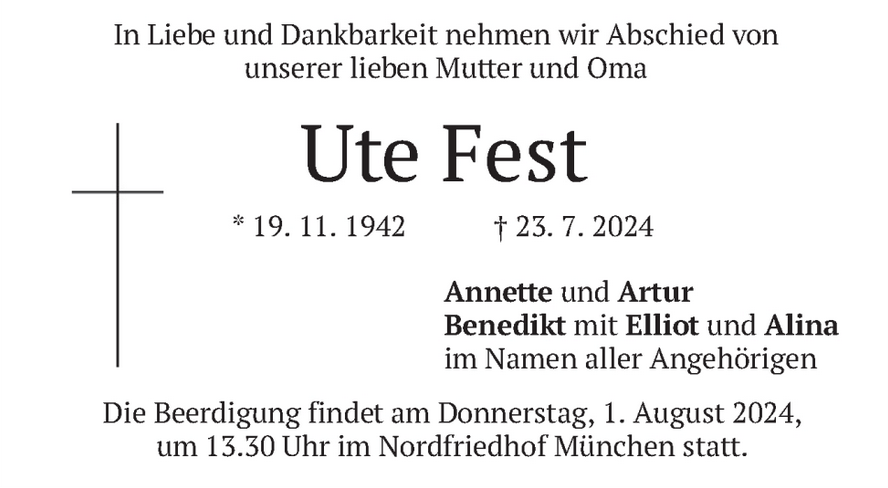
\includegraphics[width=.7\linewidth]{./Todesanzeigen/23.07.2024 Ute Fest.png}}
%		\vspace*{0.5cm}
%		\fbox{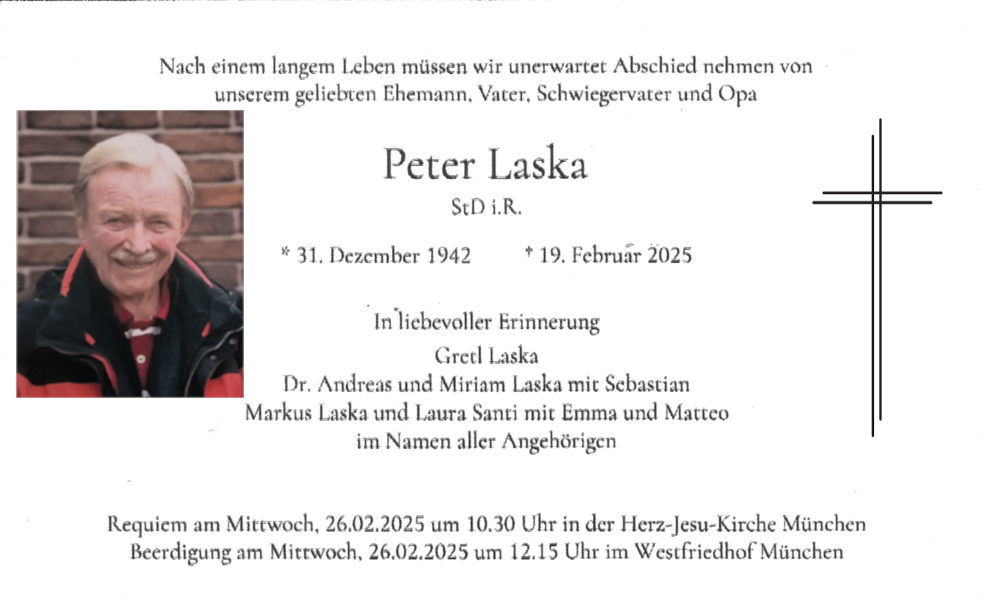
\includegraphics[width=.7\linewidth]{./Todesanzeigen/19.02.2025 PeterLaska.png}}
%	\end{center}
%\end{figure}
\begin{figure}[h!]
    \centering
    \fbox{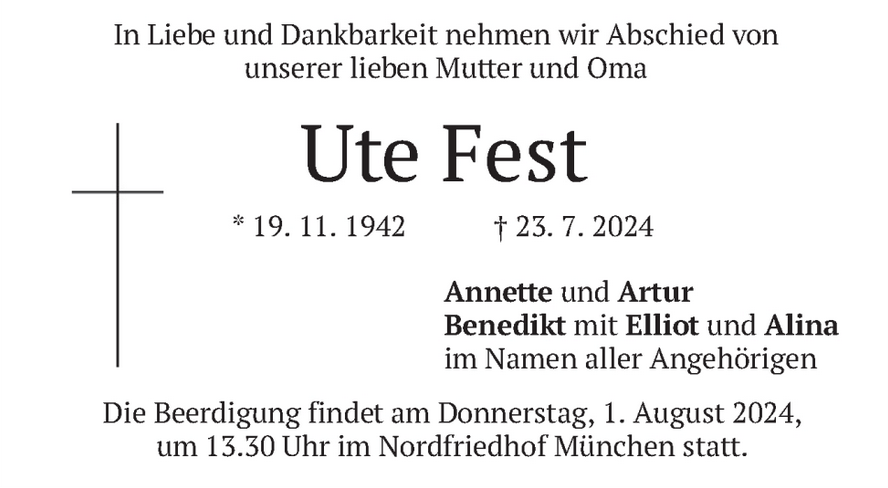
\includegraphics[width=.7\linewidth]{./Todesanzeigen/23.07.2024 Ute Fest.png}}
\end{figure}
    \vspace{0.4cm} % Should work better
\begin{figure}[h!]
    \centering
    \fbox{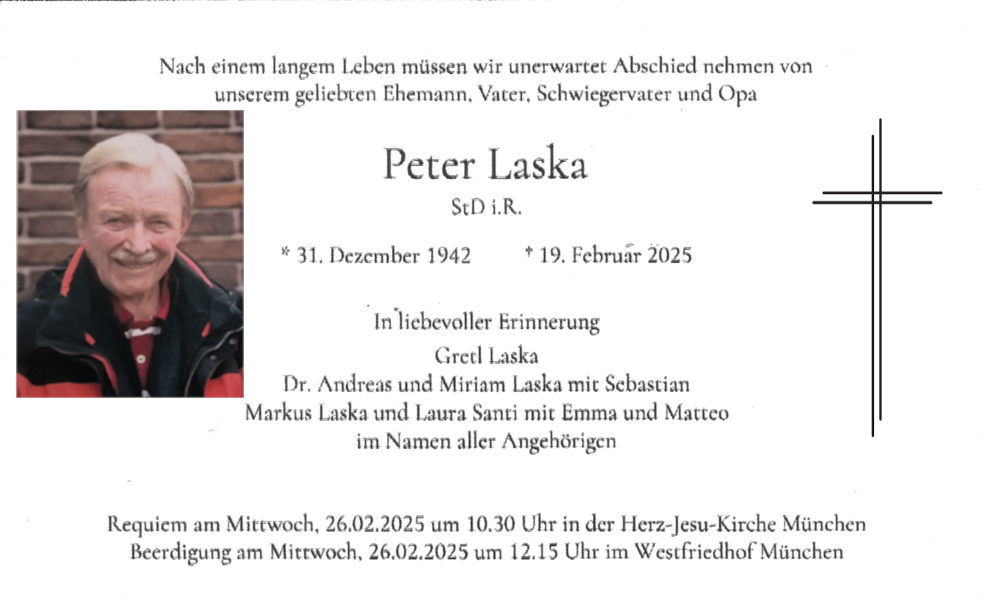
\includegraphics[width=.7\linewidth]{./Todesanzeigen/19.02.2025 PeterLaska.png}}
\end{figure}

\begin{multicols}{2}
			Am 26 Februar 2025 wurde unser Bundesbruder Peter Laska, StD i.R., im Familiengrab im Münchner Westfriedhof beigesetzt.
			Hier ruht auch sein Vater, unser hochverdienter Bundesbruder Josef Laska.
			Drei Chargierte der Aktivitas und einige Bundesbrüder erwiesen ihm die letzte Ehre und gaben ihm Band und Mütze als
			Dank und Zeichen der Verbundenheit mit ins Grab.
			Bundesbruder Peter Laska, geb. 1942 in Böhmen, wurde am 13.11.1964 von Vandalia rezipiert.
			Im WS 1965 war er Consenior der Aktivitas, 1966 Senior.
			Im Mai 1975 philistriert, übernahm er dennoch das anspruchsvolle Amt des Jubelseniors - 70 Jahre Vandalia! -
			 im Sommersemester 1975, um danach das Amt des Philisterconseniors weiterzuführen.
			61 Jahre lang hat Bbr. Peter Laska Vandalia die Treue gehalten. Ihm gebührt Vandalias besonderer Dank.
			REQUIESCAT IN PACE!
			\begin{flushright}
			\hfill\emph{Bernhard Müller Va!}
			\end{flushright}
\end{multicols}

\clearpage



%%%%%%%%%%%%%%%%%%%%%%%%%%%%%%%%%%%%%%%%%%%%%%%%%
%% Vandalia gratuliert
\section*{Vandalia gratuliert}
\sectionmark{Vandalia gratuliert}

{\footnotesize

\begin{multicols}{2}
	
%\textbf{zum 20. Geburtstag}\\


%\textbf{zum 30. Geburtstag}\\


\textbf{zum 40. Geburtstag}\\
Gabriel Lederle (12.04.1985)
\\



%\textbf{zum 50. Geburtstag}\\    Für spätere verwendung da niemand WS2024-2025 50 geworden ist




\textbf{zum 60. Geburtstag} \\
Alexander Huber (24.05.1965)\\
Stefan Guggenmos (13.05.1965)\\


% \textbf{zum 70. Geburtstag}\\ Siehe oben


%\textbf{zum 75. Geburtstag}\\ Siehe oben




\textbf{zum 80. Geburtstag}\\
Elmer Weisshuhn (10.04.1945)\\
Johann Berger (01.03.1945)\\
Wolfgang Bouché (28.02.1945)\\
Wolfgang Schorn (21.02.1945)\\

%\textbf{zum 85. Geburtstag}\\



\textbf{zum 90. Geburtstag}\\
Konrad Mayer (24.05.1935)\\
Richard  Strobel (05.05.1935)\\

\columnbreak

\textbf{zum 95. Geburtstag}\\
Ferdinand Stocker (17.03.1930) \\


%\vspace{1.5mm}

%\textbf{zur Vaterschaft}\\


\textbf{zur Hochzeit}\\
Bundesbruder Anton Brandl und seiner Frau Corina
zur Hochzeit am 28.12.2024
%\textbf{zur Geburt}\\


\vspace{1.5mm}

%\textbf{zur Philistrierung}\\


%\textbf{zur Burschung}\\


%\textbf{zur Promotion}\\

%\textbf{zum 100 Semesterband}\\

\textbf{zur Philistrierung}\\
SoSe 2023:\\
Janosch Christ\\
Martin Kölbl\\
\newline
WiSe 2023/24:\\
Philip Levi


\vspace{1.5mm}



%\textbf{ZMer im Sommersemester}\\


%\vspace{5mm}
%\vbox{
%	\textbf{Chargenkabinett des SS 20}\\[0.5ex]
%	\begin{tabular}[h]{rl}
%		X     & Korbinian Heinrich \cr
%		FM    & Felix Fisel \cr
%		XX    & Noel Riedl \cr
%		XXX   & Elias Baumgartner \cr
%		XXXX  & Andreas Mayerhofer \cr
%	\end{tabular}
%}



\end{multicols}


\vspace{1cm}

\begin{multicols}{2}

%\vspace{6pt}
%\vfill
%\vspace{12pt}
%\vspace{5pt}

\vbox{
\textbf{Chargenkabinett des WS24/25}\\[0.5ex]
\begin{tabular}[h]{rl}
	X     & Raphael Frank \cr
	FM    & Magnus Weig \cr
	XX    & Elia Strasser \cr
	XXX   & Benedikt Kirchhof \cr
	XXXX  & Felix Hantke \cr
\end{tabular}
}

\end{multicols}                                                                                       

%\vfill

%\begin{figurehere}
%  \begin{center}
%    \includegraphics[width=\hsize]{Bilder/ChC_SS11.jpg}
%    \caption{Das Chargenkabinett Vandaliae im Sommersemester 2011}
%  \end{center}
%\end{figurehere} 
}



\end{document}
